\newcommand{\sout}{}
Chapter:
CC-BY-SA 3.0
Math in Society
A survey of mathematics for the liberal arts major
Math in Society is a free, open textbook. This book is a survey of contemporary mathematical topics, most non-algebraic, appropriate for a college-level quantitative literacy topics course for liberal arts majors. The text is designed so that most chapters are independent, allowing the instructor to choose a selection of topics to be covered. Emphasis is placed on the applicability of the mathematics. Core material for each topic is covered in the main text, with additional depth available through exploration exercises appropriate for in-class, group, or individual investigation. This book is appropriate for Washington State Community Colleges' Math 107.

The current version is 2.5, released Dec 2017.
\url{http://www.opentextbookstore.com/mathinsociety/2.5/GraphTheory.pdf}

Communicated by 
Tricia Muldoon Brown, Ph.D.
Associate Professor of Mathematics
Georgia Southern University
Armstrong Campus
Savannah, GA 31419\url{http://math.armstrong.edu/faculty/brown/MATH1001.html}

\section{Graph Theory and Network Flows}
In the modern world, planning efficient routes is essential for business and industry, with applications as varied as product distribution, laying new fiber optic lines for broadband internet, and suggesting new friends within social network websites like Facebook.

This field of mathematics started nearly 300 years ago as a look into a mathematical puzzle (we'll look at it in a bit).  The field has exploded in importance in the last century, both because of the growing complexity of business in a global economy and because of the computational power that computers have provided us.  
\section{Graphs}
\subsection{Drawing Graphs}

\begin{example}
Here is a portion of a housing development from Missoula, Montana\footnote{Same Beebe. http://www.flickr.com/photos/sbeebe/2850476641/}.  As part of her job, the development's lawn inspector has to walk down every street in the development making sure homeowners' landscaping conforms to the community requirements.\\
\begin{center}
\scalebox{0.8}{
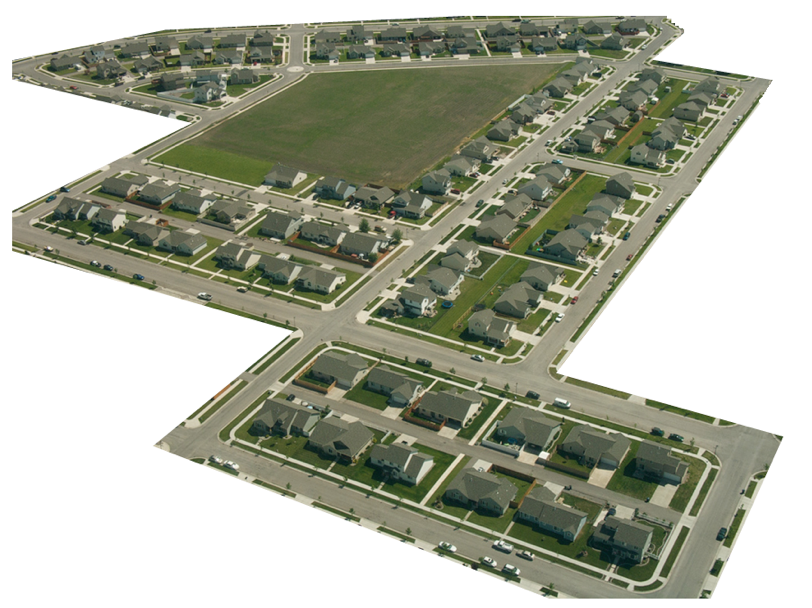
\includegraphics{graph-theory-graphics/GraphPicture.png}
}
\end{center}

Naturally, she wants to minimize the amount of walking she has to do.  Is it possible for her to walk down every street in this development without having to do any backtracking?  While you might be able to answer that question just by looking at the picture for a while, it would be ideal to be able to answer the question for any picture regardless of its complexity.\\

To do that, we first need to simplify the picture into a form that is easier to work with.  We can do that by drawing a simple line for each street.  Where streets intersect, we will place a dot. \\
 
 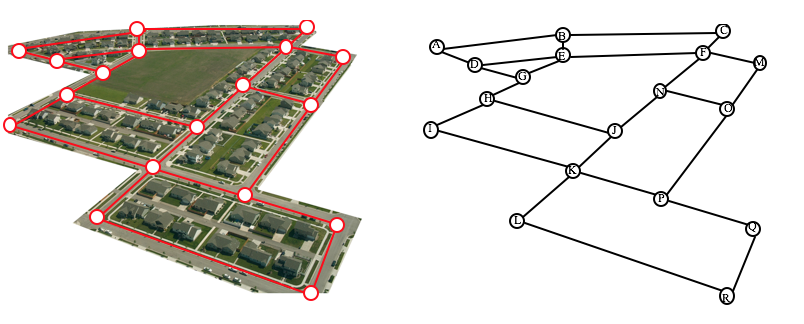
\includegraphics{graph-theory-graphics/GraphPictureDot.png}
\end{example}

This type of simplified picture is called a \textbf{graph}.  


\begin{definition}{Graphs, Vertices, and Edges}{}
A graph consists of a set of dots, called vertices, and a set of edges connecting pairs of vertices.  
\end{definition}

While we drew our original graph to correspond with the picture we had, there is nothing particularly important about the layout when we analyze a graph.  Both of the graphs below are equivalent to the one drawn above since they show the same edge connections between the same vertices as the original graph.

 
\begin{minipage}{0.5\textwidth}
\begin{tikzpicture}
    \foreach \pos/\name in {{(0,0)/A}, {(1,0)/D}, {(2,0)/G}, {(3,0)/N}, {(4,0)/O}, {(1,1)/B}, {(2,1)/E}, {(3,1)/F}, {(4,1)/M}, {(3,2)/C}, {(2,-1)/H}, {(3,-1)/J}, {(2,-2)/I}, {(3,-2)/K}, {(4,-2)/P}, {(5,-2)/Q}, {(3,-3)/L}, {(5,-3)/R}}
                \node[vertex] (\name) at \pos {$\name$};
                
 \foreach \source/ \dest in {A/D, D/G, A/B, B/E, B/C, C/F, E/F, F/M, D/E, E/G, G/H, H/I, H/J, I/K, J/K, K/L, N/J, F/N, F/M, N/O, O/P, P/Q, Q/R, M/O, K/P, L/R}
              \path (\source) edge (\dest);                
\end{tikzpicture}     
\end{minipage}
%
\begin{minipage}{0.5\textwidth}
\begin{tikzpicture}
    \foreach \pos/\name in {{(0,0)/A}, {(0,-1)/D}, {(0.6,-2.25)/G}, {(6,-1)/N}, {(3.5,2.5)/O}, {(.25,1)/B}, {(5.4,1.25)/E}, {(2.4,-3.5)/F}, {(4.6,2.25)/M}, {(1,1.75)/C}, {(1.4,-3.25)/H}, {(5.75,-2)/J}, {(6,0)/I}, {(3.5,-3.5)/K}, {(2.5,2.5)/P}, {(1.6,2.25)/Q}, {(4.4,-3.25)/L}, {(5,-2.75)/R}}
                \node[vertex] (\name) at \pos {$\name$};
                
 \foreach \source/ \dest in {A/D, D/G, A/B, B/E, B/C, C/F, E/F, F/M, D/E, E/G, G/H, H/I, H/J, I/K, J/K, K/L, N/J, F/N, F/M, N/O, O/P, P/Q, Q/R, M/O, K/P, L/R}
              \path (\source) edge (\dest);                
\end{tikzpicture}   
\end{minipage}

You probably already noticed that we are using the term graph differently than you may have used the term in the past to describe the graph of a mathematical function.


\begin{example}{}{}

Back in the 18th century in the Prussian city of K\"onigsberg, a river ran through the city and seven bridges crossed the forks of the river.  The river and the bridges are highlighted in the picture to the right%\footnote{Bogdan Giusc\u{a}. \url{http://en.wikipedia.org/wiki/File:Konigsberg\_bridges.png}}.

\textcolor{red}{Picture}

As a weekend amusement, townsfolk would see if they could find a route that would take them across every bridge once and return them to where they started.

Leonard Euler (pronounced OY-lur), one of the most prolific mathematicians ever, looked at this problem in 1735, laying the foundation for graph theory as a field in mathematics.  To analyze this problem, Euler introduced edges representing the bridges:
\begin{center}
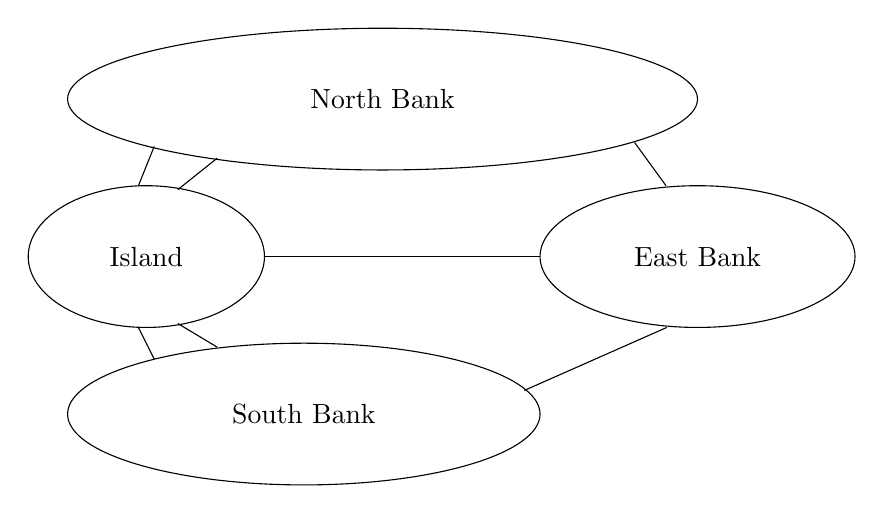
\begin{tikzpicture}
\draw (2,2) ellipse (4cm and .9cm); %NB
\node at (2,2) {North Bank};
\draw (-1,0) ellipse (1.5cm and .9cm); %I
\node at (-1,0) {Island};
\draw (6,0) ellipse (2cm and .9cm); %EB
\node at (6,0) {East Bank};
\draw (1,-2) ellipse (3cm and .9cm);
\node at (1,-2) {South Bank};
\draw(-1.1,.9)--(-.9,1.4);
\draw(-.6,.85)--(-.1,1.25);
\draw(-1.1,-.9)--(-.9,-1.3);
\draw(-.6,-.85)--(-.1,-1.15);
\draw(0.5,0)--(4,0);
\draw(5.6,0.9)--(5.2,1.45);
\draw(5.61,-0.9)--(3.8,-1.7);
\end{tikzpicture}
\end{center}
Since the size of each land mass it is not relevant to the question of bridge crossings, each can be shrunk down to a vertex representing the location:
\begin{center}
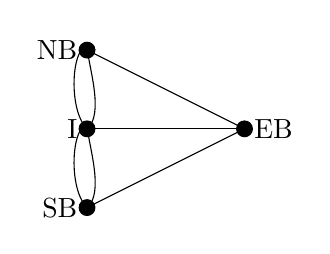
\begin{tikzpicture}
\draw(0,1)--(2,1);
\draw(0,2)--(2,1);
\draw(0,0)--(2,1);
\draw(0,0) to [out=40] (0.1,1);
\draw(0,0) to [out=135] (0.1,1);
\draw(0,1) to [out=40] (0.1,2);
\draw(0,1) to [out=135] (0.1,2);
\draw[fill] (0,0) circle[radius=.1] node [left]{SB};
\draw[fill] (0,1) circle[radius=.1] node [left]{I   };
\draw[fill] (0,2) circle[radius=.1] node [left]{NB};
\draw[fill] (2,1) circle[radius=.1] node [right]{EB};
\end{tikzpicture}
\end{center}

Notice that in this graph there are \textit{two} edges connecting the north bank and island, corresponding to the two bridges in the original drawing.  Depending upon the interpretation of edges and vertices appropriate to a scenario, it is entirely possible and reasonable to have more than one edge connecting two vertices.

While we haven't answered the actual question yet of whether or not there is a route which crosses every bridge once and returns to the starting location, the graph provides the foundation for exploring this question.
 \end{example}


\section{Definitions}
While we loosely defined some terminology earlier, we now will try to be more specific.

\begin{definition}{Vertex}{vertex} 
A vertex is a dot in the graph that could represent an intersection of streets, a land mass, or a general location, like ``work? or ``school".  Vertices are often connected by edges.  Note that vertices only occur when a dot is explicitly placed, not whenever two edges cross.  Imagine a freeway overpass -- the freeway and side street cross, but it is not possible to change from the side street to the freeway at that point, so there is no intersection and no vertex would be placed.
\end{definition}

\begin{definition}{Edges}{}
Edges connect pairs of vertices.  An edge can represent a physical connection between locations, like a street, or simply that a route connecting the two locations exists, like an airline flight.
\end{definition}

\begin{definition}{Loop}{}
A loop is a special type of edge that connects a vertex to itself.  Loops are not used much in street network graphs.\\

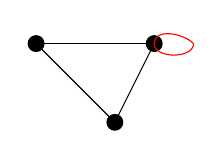
\begin{tikzpicture}
\draw[fill] (0,0) circle[radius=.1];
\draw[fill] (1,-1) circle[radius=.1];
\draw[fill] (1.5,0) circle[radius=.1];
\draw(0,0)--(1,-1);
\draw(0,0)--(1.5,0);
\draw(1.5,0)--(1,-1);  
 \draw[red](1.5,0) to [out=90] (2,0);
 \draw[red](1.5,0) to [out=-90, in=-90] (2,0);
 \end{tikzpicture}
 \end{definition}


\begin{definition}{Degree of a vertex}{}
The degree of a vertex is the number of edges meeting at that vertex.  It is possible for a vertex to have a degree of zero or larger.
\begin{center}
\begin{tabular}{|c|c|c|c|c|}
\hline
Degree 0 & Degree 1 & Degree 2 & Degree 3 & Degree 4\\
\hline

\begin{tikzpicture}
\draw[fill] (0,0) circle[radius=.1];
\node at (0,-1){};
\end{tikzpicture}
&
\begin{tikzpicture}
\draw[fill] (0,0) circle[radius=.1];
\draw(0,0)--(1,1);
\node at (-.6,-1){};
\node at (1,1){};
\end{tikzpicture}
&
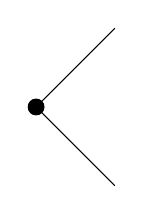
\begin{tikzpicture}
\draw[fill] (0,0) circle[radius=.1];
\draw(0,0)--(1,1);
\draw(0,0)--(1,-1);
\end{tikzpicture}
&
\begin{tikzpicture}
\draw[fill] (0,0) circle[radius=.1];
\draw(0,0)--(1,1);
\draw(0,0)--(1,-1);
\draw(0,0)--(-1,1);
\end{tikzpicture}
&
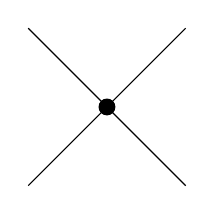
\begin{tikzpicture}
\draw[fill] (0,0) circle[radius=.1];
\draw(0,0)--(1,1);
\draw(0,0)--(1,-1);
\draw(0,0)--(-1,1);
\draw(0,0)--(-1,-1);
\end{tikzpicture}\\
\hline
\end{tabular}
\end{center}
 
 \end{definition}



\begin{definition}{Path}{}
A path is a sequence of vertices using the edges.  Usually we are interested in a path between two vertices.  For example, a path from vertex A to vertex M is shown below.  It is one of many possible paths in this graph. 

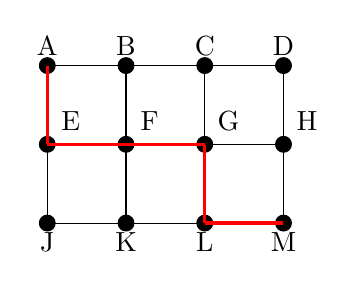
\begin{tikzpicture}
\draw[fill] (0,2) circle[radius=.1] node[above]{A};
\draw[fill] (1,2) circle[radius=.1] node[above]{B};
\draw[fill] (2,2) circle[radius=.1] node[above]{C};
\draw[fill] (3,2) circle[radius=.1] node[above]{D};
\draw[fill] (0,1) circle[radius=.1];
\node at (0.3,1.3){E}; 
\draw[fill] (1,1) circle[radius=.1];
\node at (1.3,1.3){F}; 
\draw[fill] (2,1) circle[radius=.1];
\node at (2.3,1.3){G};  
\draw[fill] (3,1) circle[radius=.1];
\node at (3.3,1.3){H};  
\draw[fill] (0,0) circle[radius=.1] node[below]{J};
\draw[fill] (1,0) circle[radius=.1] node[below]{K};
\draw[fill] (2,0) circle[radius=.1] node[below]{L};
\draw[fill] (3,0) circle[radius=.1] node[below]{M};
\draw(0,0)--(0,1);
\draw[very thick, red](0,1)--(0,2);
\draw(1,0)--(1,1);
\draw(1,1)--(1,2);
\draw[very thick, red](2,0)--(2,1);
\draw(2,1)--(2,2);
\draw(3,0)--(3,1);
\draw(3,1)--(3,2);
\draw(0,0)--(1,0);
\draw(1,0)--(2,0);
\draw[very thick, red](2,0)--(3,0);
\draw[very thick, red](0,1)--(1,1);
\draw[very thick, red](1,1)--(2,1);
\draw(2,1)--(3,1);
\draw(0,2)--(1,2);
\draw(1,2)--(2,2);
\draw(2,2)--(3,2);
\end{tikzpicture}

 \end{definition}



\begin{definition}{Circuit}{}
A circuit is a path that begins and ends at the same vertex.  A circuit starting and ending at vertex A is shown below.

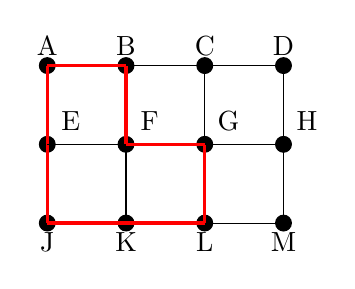
\begin{tikzpicture}
\draw[fill] (0,2) circle[radius=.1] node[above]{A};
\draw[fill] (1,2) circle[radius=.1] node[above]{B};
\draw[fill] (2,2) circle[radius=.1] node[above]{C};
\draw[fill] (3,2) circle[radius=.1] node[above]{D};
\draw[fill] (0,1) circle[radius=.1];
\node at (0.3,1.3){E}; 
\draw[fill] (1,1) circle[radius=.1];
\node at (1.3,1.3){F}; 
\draw[fill] (2,1) circle[radius=.1];
\node at (2.3,1.3){G};  
\draw[fill] (3,1) circle[radius=.1];
\node at (3.3,1.3){H};  
\draw[fill] (0,0) circle[radius=.1] node[below]{J};
\draw[fill] (1,0) circle[radius=.1] node[below]{K};
\draw[fill] (2,0) circle[radius=.1] node[below]{L};
\draw[fill] (3,0) circle[radius=.1] node[below]{M};
\draw[very thick, red](0,0)--(0,1);
\draw[very thick, red](0,1)--(0,2);
\draw(1,0)--(1,1);
\draw[very thick, red](1,1)--(1,2);
\draw[very thick, red](2,0)--(2,1);
\draw(2,1)--(2,2);
\draw(3,0)--(3,1);
\draw(3,1)--(3,2);
\draw[very thick, red](0,0)--(1,0);
\draw[very thick, red](1,0)--(2,0);
\draw(2,0)--(3,0);
\draw(0,1)--(1,1);
\draw[very thick, red](1,1)--(2,1);
\draw(2,1)--(3,1);
\draw[very thick, red](0,2)--(1,2);
\draw(1,2)--(2,2);
\draw(2,2)--(3,2);
\end{tikzpicture}

\end{definition}




\begin{definition}{Connected}{}
A graph is connected if there is a path from any vertex to any other vertex.  Every graph drawn so far has been connected.  The graph below is \textbf{disconnected}; there is no way to get from the vertices on the left to the vertices on the right.

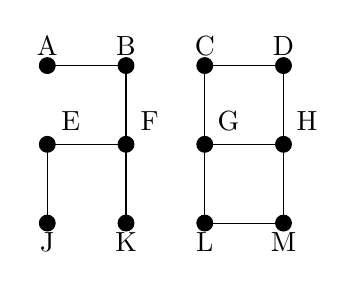
\begin{tikzpicture}
\draw[fill] (0,2) circle[radius=.1] node[above]{A};
\draw[fill] (1,2) circle[radius=.1] node[above]{B};
\draw[fill] (2,2) circle[radius=.1] node[above]{C};
\draw[fill] (3,2) circle[radius=.1] node[above]{D};
\draw[fill] (0,1) circle[radius=.1];
\node at (0.3,1.3){E}; 
\draw[fill] (1,1) circle[radius=.1];
\node at (1.3,1.3){F}; 
\draw[fill] (2,1) circle[radius=.1];
\node at (2.3,1.3){G};  
\draw[fill] (3,1) circle[radius=.1];
\node at (3.3,1.3){H};  
\draw[fill] (0,0) circle[radius=.1] node[below]{J};
\draw[fill] (1,0) circle[radius=.1] node[below]{K};
\draw[fill] (2,0) circle[radius=.1] node[below]{L};
\draw[fill] (3,0) circle[radius=.1] node[below]{M};
\draw(0,0)--(0,1);
\draw(1,0)--(1,1);
\draw(1,1)--(1,2);
\draw(2,0)--(2,1);
\draw(2,1)--(2,2);
\draw(3,0)--(3,1);
\draw(3,1)--(3,2);
\draw(2,0)--(3,0);
\draw(0,1)--(1,1);

\draw(2,1)--(3,1);
\draw(0,2)--(1,2);
\draw(2,2)--(3,2);
\end{tikzpicture}
 \end{definition}





\begin{definition}{Weights}{}
Depending upon the problem being solved, sometimes weights are assigned to the edges.  The weights could represent the distance between two locations, the travel time, or the travel cost.  It is important to note that the distance between vertices in a graph does not necessarily correspond to the weight of an edge.
 \end{definition}

\begin{exercise}{}{}
The graph below shows 5 cities.  The weights on the edges represent the airfare for a one-way flight between the cities.
 \begin{enumerate}[label=\alph*.]
 \item How many vertices and edges does the graph have?
 \item Is the graph connected?
 \item What is the degree of the vertex representing LA?
 \item If you fly from Seattle to Dallas to Atlanta, is that a path or a circuit?
 \item If you fly from LA to Chicago to Dallas to LA, is that a path or a circuit?
 \end{enumerate}
 
 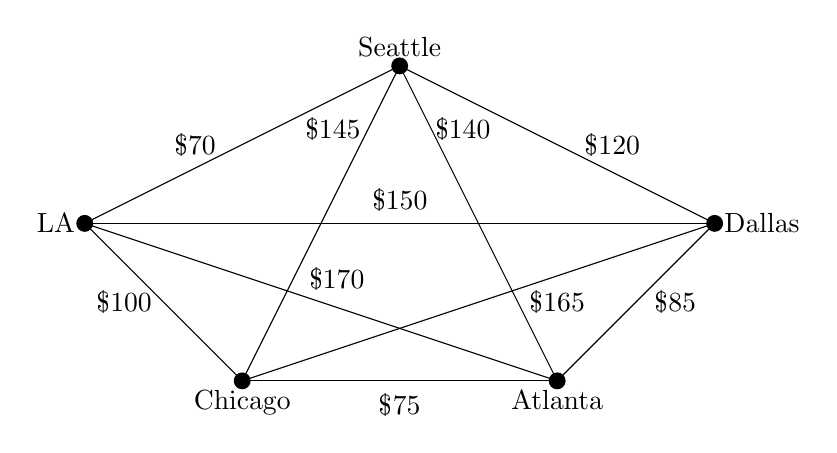
\begin{tikzpicture}
 \draw[fill] (0,0) circle[radius=.1] node[left]{LA};
\draw[fill] (2,-2) circle[radius=.1] node[below]{Chicago};
\draw[fill] (4,2) circle[radius=.1] node[above]{Seattle};
\draw[fill] (6,-2) circle[radius=.1] node[below]{Atlanta};
\draw[fill] (8,0) circle[radius=.1] node[right]{Dallas};
\draw(0,0)--(2,-2);
\node at (0.5,-1){\$100};
\draw(0,0)--(4,2);
\node at (1.4,1){\$70};
\draw(0,0)--(8,0);
\node at (4,0.3){\$150};
\draw(0,0)--(6,-2);
\node at (3.2,-0.7){\$170};
\draw(2,-2)--(4,2);
\node at (3.15,1.2){\$145};
\draw(4,2)--(6,-2);
\node at (4.8, 1.2){\$140};
\draw(4,2)--(8,0);
\node at (6.7,1){\$120};
\draw(2,-2)--(8,0);
\node at (6,-1){\$165};
\draw(2,-2)--(6,-2);
\node at (4,-2.3){\$75};
\draw(6,-2)--(8,0);
\node at (7.5,-1){\$85};
 \end{tikzpicture}
 \end{exercise}


\section{Shortest Path}
When you visit a website like Google Maps or use your Smartphone to ask for directions from home to your Aunt's house in Pasadena, you are usually looking for a shortest path between the two locations.  These computer applications use representations of the street maps as graphs, with estimated driving times as edge weights.

While often it is possible to find a shortest path on a small graph by guess-and-check, our goal in this chapter is to develop methods to solve complex problems in a systematic way by following \textbf{algorithms}.  An algorithm is a step-by-step procedure for solving a problem.  Dijkstra's (pronounced dike-stra) algorithm will find the shortest path between two vertices.


\begin{algorithm}{Dijkstra's Algorithm}{}
\hspace{3in}

\begin{enumerate}
\item	Mark the ending vertex with a distance of zero.  Designate this vertex as current.
\item Find all vertices leading to the current vertex.  Calculate their distances to the end.  Since we already know the distance the current vertex is from the end, this will just require adding the most recent edge.  Don't record this distance if it is longer than a previously recorded distance.
\item	Mark the current vertex as visited.  We will never look at this vertex again.
\item	Mark the vertex with the smallest distance as current, and repeat from step 2.
\end{enumerate}
 \end{algorithm}

\newpage
\begin{example}{}{}
Suppose you need to travel from Tacoma, WA (vertex T) to Yakima, WA (vertex Y).  Looking at a map, it looks like driving through Auburn (A) then Mount Rainier (MR) might be shortest, but it's not totally clear since that road is probably slower than taking the major highway through North Bend (NB).  A graph with travel times in minutes is shown below.  An alternate route through Eatonville (E) and Packwood (P) is also shown.

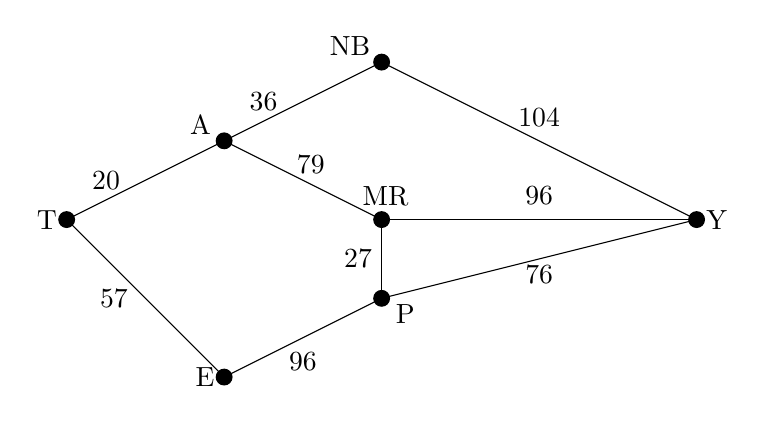
\begin{tikzpicture}
\draw[fill] (0,0) circle[radius=.1] node[left]{T};
\draw[fill] (2,-2) circle[radius=.1] node[left]{E};
\draw[fill] (2,1) circle[radius=.1];
\node at (1.7,1.2){A};
\draw[fill] (4,2) circle[radius=.1]; 
\node at (3.6,2.2){NB};
\draw[fill] (4,0) circle[radius=.1];
\node at (4.05,0.3){MR};
\draw[fill] (4,-1) circle[radius=.1];
\node at (4.3,-1.2){P};
\draw[fill] (8,0) circle[radius=.1] node[right]{Y};
\draw(0,0)--(2,-2);
\node at (0.6,-1){57};
\draw(0,0)--(2,1);
\node at (0.5, 0.5){20};
\draw(2,1)--(4,2);
\node at (2.5,1.5){36};
\draw(4,2)--(8,0);
\node at (6,1.3){104};
\draw(2,-2)--(4,-1);
\node at (3,-1.8){96};
\draw(4,-1)--(8,0);
\node at (6,-0.7){76};
\draw(2,1)--(4,0);
\node at (3.1,0.7){79};
\draw(4,0)--(4,-1);
\node at (3.7, -0.5){27};
\draw(4,0)--(8,0);
\node at (6,0.3){96};
\end{tikzpicture}







\noindent Step 1:  Mark the ending vertex with a distance of zero.  The distances will be recorded in [brackets] after the vertex name.\\
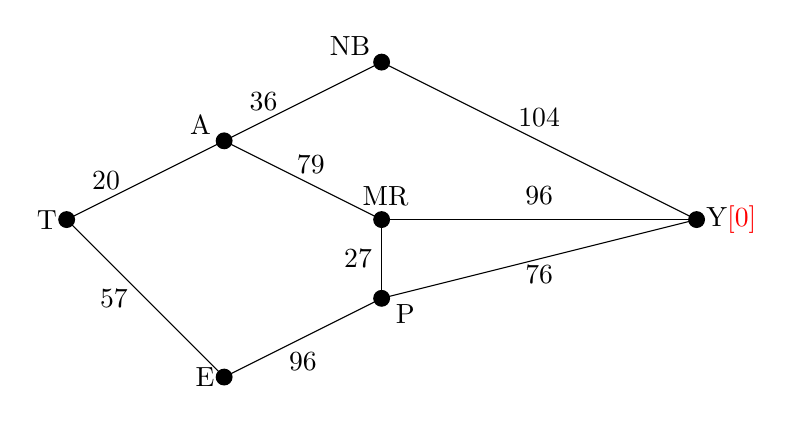
\begin{tikzpicture}
\draw[fill] (0,0) circle[radius=.1] node[left]{T};
\draw[fill] (2,-2) circle[radius=.1] node[left]{E};
\draw[fill] (2,1) circle[radius=.1];
\node at (1.7,1.2){A};
\draw[fill] (4,2) circle[radius=.1]; 
\node at (3.6,2.2){NB};
\draw[fill] (4,0) circle[radius=.1];
\node at (4.05,0.3){MR};
\draw[fill] (4,-1) circle[radius=.1];
\node at (4.3,-1.2){P};
\draw[fill] (8,0) circle[radius=.1] node[right]{Y\textcolor{red}{[0]}};
\draw(0,0)--(2,-2);
\node at (0.6,-1){57};
\draw(0,0)--(2,1);
\node at (0.5, 0.5){20};
\draw(2,1)--(4,2);
\node at (2.5,1.5){36};
\draw(4,2)--(8,0);
\node at (6,1.3){104};
\draw(2,-2)--(4,-1);
\node at (3,-1.8){96};
\draw(4,-1)--(8,0);
\node at (6,-0.7){76};
\draw(2,1)--(4,0);
\node at (3.1,0.7){79};
\draw(4,0)--(4,-1);
\node at (3.7, -0.5){27};
\draw(4,0)--(8,0);
\node at (6,0.3){96};
\end{tikzpicture}


\noindent Step 2:  For each vertex leading to Y, we calculate the distance to the end.  For example, NB is a distance of 104 from the end, and MR is 96 from the end.  Remember that distances in this case refer to the travel time in minutes.\\
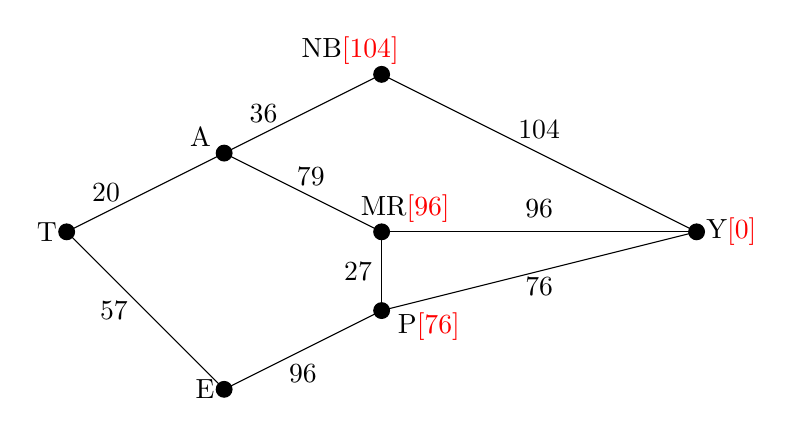
\begin{tikzpicture}
\draw[fill] (0,0) circle[radius=.1] node[left]{T};
\draw[fill] (2,-2) circle[radius=.1] node[left]{E};
\draw[fill] (2,1) circle[radius=.1];
\node at (1.7,1.2){A};
\draw[fill] (4,2) circle[radius=.1]; 
\node at (3.6,2.3){NB\textcolor{red}{[104]}};
\draw[fill] (4,0) circle[radius=.1];
\node at (4.3,0.3){MR\textcolor{red}{[96]}};
\draw[fill] (4,-1) circle[radius=.1];
\node at (4.6,-1.2){P\textcolor{red}{[76]}};
\draw[fill] (8,0) circle[radius=.1] node[right]{Y\textcolor{red}{[0]}};
\draw(0,0)--(2,-2);
\node at (0.6,-1){57};
\draw(0,0)--(2,1);
\node at (0.5, 0.5){20};
\draw(2,1)--(4,2);
\node at (2.5,1.5){36};
\draw(4,2)--(8,0);
\node at (6,1.3){104};
\draw(2,-2)--(4,-1);
\node at (3,-1.8){96};
\draw(4,-1)--(8,0);
\node at (6,-0.7){76};
\draw(2,1)--(4,0);
\node at (3.1,0.7){79};
\draw(4,0)--(4,-1);
\node at (3.7, -0.5){27};
\draw(4,0)--(8,0);
\node at (6,0.3){96};
\end{tikzpicture}


\noindent Step 3 \& 4:  We mark Y as visited, and mark the vertex with the smallest recorded distance as current.  At this point, P will be designated current.  Back to step 2.\\

\newpage
\noindent Step 2 (\#2):  For each vertex leading to P (and not leading to a visited vertex) we find the distance from the end.  Since E is 96 minutes from P, and we've already calculated P is 76 minutes from Y, we can compute that E is $96+76 = 172$ minutes from Y.  \\

If we make the same computation for MR, we'd calculate $76+27 = 103$.  Since this is larger than the previously recorded distance from Y to MR, we will not replace it.\\
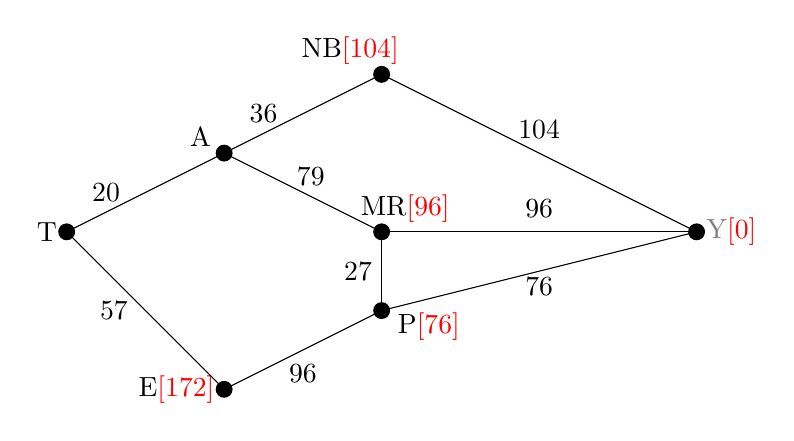
\begin{tikzpicture}
\draw[fill] (0,0) circle[radius=.1] node[left]{T};
\draw[fill] (2,-2) circle[radius=.1] node[left]{E\textcolor{red}{[172]}};
\draw[fill] (2,1) circle[radius=.1];
\node at (1.7,1.2){A};
\draw[fill] (4,2) circle[radius=.1]; 
\node at (3.6,2.3){NB\textcolor{red}{[104]}};
\draw[fill] (4,0) circle[radius=.1];
\node at (4.3,0.3){MR\textcolor{red}{[96]}};
\draw[fill] (4,-1) circle[radius=.1];
\node at (4.6,-1.2){P\textcolor{red}{[76]}};
\draw[fill] (8,0) circle[radius=.1] node[right]{\textcolor{gray}{\sout{Y}}\textcolor{red}{[0]}};
\draw(0,0)--(2,-2);
\node at (0.6,-1){57};
\draw(0,0)--(2,1);
\node at (0.5, 0.5){20};
\draw(2,1)--(4,2);
\node at (2.5,1.5){36};
\draw(4,2)--(8,0);
\node at (6,1.3){104};
\draw(2,-2)--(4,-1);
\node at (3,-1.8){96};
\draw(4,-1)--(8,0);
\node at (6,-0.7){76};
\draw(2,1)--(4,0);
\node at (3.1,0.7){79};
\draw(4,0)--(4,-1);
\node at (3.7, -0.5){27};
\draw(4,0)--(8,0);
\node at (6,0.3){96};
\end{tikzpicture}



\noindent Step 3 \& 4 (\#2):  We mark P as visited, and designate the vertex with the smallest recorded distance as current:  MR.  Back to step 2.\\

\noindent Step 2 (\#3):  For each vertex leading to MR (and not leading to a visited vertex) we find the distance to the end.  The only vertex to be considered is A, since we've already visited Y and P.  Adding MR's distance 96 to the length from A to MR gives the distance $96+79 = 175$ minutes from A to Y.  \\
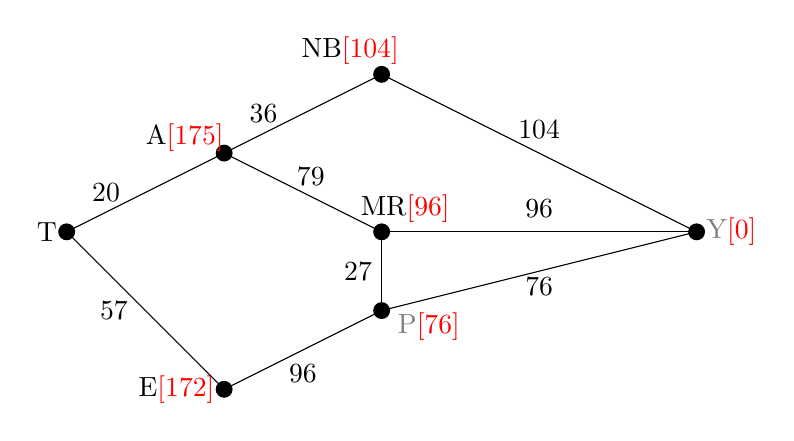
\begin{tikzpicture}
\draw[fill] (0,0) circle[radius=.1] node[left]{T};
\draw[fill] (2,-2) circle[radius=.1] node[left]{E\textcolor{red}{[172]}};
\draw[fill] (2,1) circle[radius=.1];
\node at (1.5,1.2){A\textcolor{red}{[175]}};
\draw[fill] (4,2) circle[radius=.1]; 
\node at (3.6,2.3){NB\textcolor{red}{[104]}};
\draw[fill] (4,0) circle[radius=.1];
\node at (4.3,0.3){MR\textcolor{red}{[96]}};
\draw[fill] (4,-1) circle[radius=.1];
\node at (4.6,-1.2){\textcolor{gray}{\sout{P}}\textcolor{red}{[76]}};
\draw[fill] (8,0) circle[radius=.1] node[right]{\textcolor{gray}{\sout{Y}}\textcolor{red}{[0]}};
\draw(0,0)--(2,-2);
\node at (0.6,-1){57};
\draw(0,0)--(2,1);
\node at (0.5, 0.5){20};
\draw(2,1)--(4,2);
\node at (2.5,1.5){36};
\draw(4,2)--(8,0);
\node at (6,1.3){104};
\draw(2,-2)--(4,-1);
\node at (3,-1.8){96};
\draw(4,-1)--(8,0);
\node at (6,-0.7){76};
\draw(2,1)--(4,0);
\node at (3.1,0.7){79};
\draw(4,0)--(4,-1);
\node at (3.7, -0.5){27};
\draw(4,0)--(8,0);
\node at (6,0.3){96};
\end{tikzpicture}


\noindent Step 3 \& 4 (\#3):  We mark MR as visited, and designate the vertex with smallest recorded distance as current: NB.  Back to step 2.\\

\noindent Step 2 (\#4):  For each vertex leading to NB, we find the distance to the end.  We know the shortest distance from NB to Y is 104 and the distance from A to NB is 36, so the distance from A to Y through NB is $104+36 = 140$.  Since this distance is shorter than the previously calculated distance from Y to A through MR, we replace it.\\
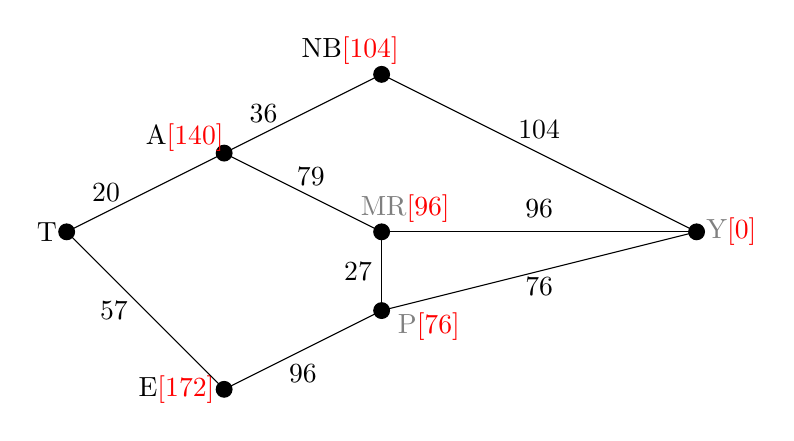
\begin{tikzpicture}
\draw[fill] (0,0) circle[radius=.1] node[left]{T};
\draw[fill] (2,-2) circle[radius=.1] node[left]{E\textcolor{red}{[172]}};
\draw[fill] (2,1) circle[radius=.1];
\node at (1.5,1.2){A\textcolor{red}{[140]}};
\draw[fill] (4,2) circle[radius=.1]; 
\node at (3.6,2.3){NB\textcolor{red}{[104]}};
\draw[fill] (4,0) circle[radius=.1];
\node at (4.3,0.3){\textcolor{gray}{\sout{MR}}\textcolor{red}{[96]}};
\draw[fill] (4,-1) circle[radius=.1];
\node at (4.6,-1.2){\textcolor{gray}{\sout{P}}\textcolor{red}{[76]}};
\draw[fill] (8,0) circle[radius=.1] node[right]{\textcolor{gray}{\sout{Y}}\textcolor{red}{[0]}};
\draw(0,0)--(2,-2);
\node at (0.6,-1){57};
\draw(0,0)--(2,1);
\node at (0.5, 0.5){20};
\draw(2,1)--(4,2);
\node at (2.5,1.5){36};
\draw(4,2)--(8,0);
\node at (6,1.3){104};
\draw(2,-2)--(4,-1);
\node at (3,-1.8){96};
\draw(4,-1)--(8,0);
\node at (6,-0.7){76};
\draw(2,1)--(4,0);
\node at (3.1,0.7){79};
\draw(4,0)--(4,-1);
\node at (3.7, -0.5){27};
\draw(4,0)--(8,0);
\node at (6,0.3){96};
\end{tikzpicture}

\noindent Step 3 \& 4 (\#4):  We mark NB as visited, and designate A as current, since it now has the shortest distance.\\


\noindent Step 2 (\#5):  T is the only non-visited vertex leading to A, so we calculate the distance from T to Y through A:  $20+140 = 160$ minutes.  \\
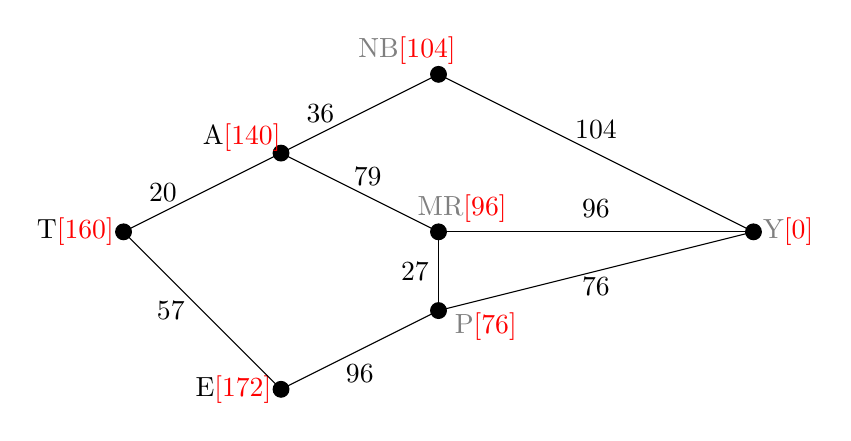
\begin{tikzpicture}
\draw[fill] (0,0) circle[radius=.1] node[left]{T\textcolor{red}{[160]}};
\draw[fill] (2,-2) circle[radius=.1] node[left]{E\textcolor{red}{[172]}};
\draw[fill] (2,1) circle[radius=.1];
\node at (1.5,1.2){A\textcolor{red}{[140]}};
\draw[fill] (4,2) circle[radius=.1]; 
\node at (3.6,2.3){\textcolor{gray}{\sout{NB}}\textcolor{red}{[104]}};
\draw[fill] (4,0) circle[radius=.1];
\node at (4.3,0.3){\textcolor{gray}{\sout{MR}}\textcolor{red}{[96]}};
\draw[fill] (4,-1) circle[radius=.1];
\node at (4.6,-1.2){\textcolor{gray}{\sout{P}}\textcolor{red}{[76]}};
\draw[fill] (8,0) circle[radius=.1] node[right]{\textcolor{gray}{\sout{Y}}\textcolor{red}{[0]}};
\draw(0,0)--(2,-2);
\node at (0.6,-1){57};
\draw(0,0)--(2,1);
\node at (0.5, 0.5){20};
\draw(2,1)--(4,2);
\node at (2.5,1.5){36};
\draw(4,2)--(8,0);
\node at (6,1.3){104};
\draw(2,-2)--(4,-1);
\node at (3,-1.8){96};
\draw(4,-1)--(8,0);
\node at (6,-0.7){76};
\draw(2,1)--(4,0);
\node at (3.1,0.7){79};
\draw(4,0)--(4,-1);
\node at (3.7, -0.5){27};
\draw(4,0)--(8,0);
\node at (6,0.3){96};
\end{tikzpicture}


\noindent Step 3 \& 4 (\#5):  We mark A as visited, and designate E as current.\\

\noindent Step 2 (\#6):  The only non-visited vertex leading to E is T.  Calculating the distance from T to Y through E, we compute $172+57 = 229$ minutes.  Since this is longer than the existing marked time, we do not replace it.  \\

\noindent Step 3 (\#6):  We mark E as visited.  Since all vertices have been visited, we are done.  \\

From this, we know that the shortest path from Tacoma to Yakima will take 160 minutes.  Tracking which sequence of edges yielded 160 minutes, we see the shortest path is T-A-NB-Y. 
\end{example}

Dijkstra's algorithm is an \textbf{optimal algorithm}, meaning that it always produces the actual shortest path, not just a path that is pretty short, provided one exists.  This algorithm is also \textbf{efficient}, meaning that it can be implemented in a reasonable amount of time.  Dijkstra's algorithm takes around V$^2$ calculations, where V is the number of vertices in a graph\footnote{It can be made to run faster through various optimizations to the implementation.}.  A graph with 100 vertices would take around 10,000 calculations.  While that would be a lot to do by hand, it is not a lot for computer to handle.  It is because of this efficiency that your car's GPS unit can compute driving directions in only a few seconds.  
 
In contrast, an \textbf{inefficient} algorithm might try to list all possible paths then compute the length of each path.  Trying to list all possible paths could easily take 10$^25$ calculations to compute the shortest path with only 25 vertices; that's a 1 with 25 zeros after it!  To put that in perspective, the fastest computer in the world would still spend over 1000 years analyzing all those paths.


\begin{example}{}{}
A shipping company needs to route a package from Washington, D.C. to San Diego, CA.  To minimize costs, the package will first be sent to their processing center in Baltimore, MD then sent as part of mass shipments between their various processing centers, ending up in their processing center in Bakersfield, CA.  From there it will be delivered in a small truck to San Diego.  

The travel times, in hours, between their processing centers are shown in the table below.  Three hours has been added to each travel time for processing.  Find the shortest path from Baltimore to Bakersfield.
 \begin{center}
 \begin{tabular}{|l|c|c|c|c|c|c|}
 \hline
 & Baltimore & Denver & Dallas & Chicago & Atlanta & Bakersfield\\
 &&&&&&\\
 \hline
 Baltimore & * &&&15&14&\\
 \hline
 Denver &&*&&18&24&19\\
 \hline
Dallas&&&*&18&15&25\\
 \hline
 Chicago &15&18&18&*&14&\\
 \hline
 Atlanta & 14 & 24&15&14&8&\\
 \hline
 Bakersfield &&19&25&&&*\\
 \hline
 \end{tabular}
 \end{center}


While we could draw a graph, we can also work directly from the table. \\

\noindent Step 1:  The ending vertex, Bakersfield, is marked as current.\\

\noindent Step 2:  All cities connected to Bakersfield, in this case Denver and Dallas, have their distances calculated; we?ll mark those distances in the column headers.  \\

\noindent Step 3 \& 4:  Mark Bakersfield as visited.  Here, we are doing it by shading the corresponding row and column of the table.  We mark Denver as current, shown in bold, since it is the vertex with the shortest distance.
 \begin{center}
 \begin{tabular}{|l|c|c|c|c|c|c|}
 \hline
 & Baltimore & \textbf{Denver} & Dallas & Chicago & Atlanta & \cellcolor{yellow}Bakersfield\\
 &&[19]&[25]&&&\cellcolor{yellow}[0]\\
 \hline
 Baltimore & * &&&15&14&\cellcolor{yellow}\\
 \hline
 Denver &&*&&18&24&\cellcolor{yellow}19\\
 \hline
Dallas&&&*&18&15&\cellcolor{yellow}25\\
 \hline
 Chicago &15&18&18&*&14&\cellcolor{yellow}\\
 \hline
 Atlanta & 14 & 24&15&14&8&\cellcolor{yellow}\\
 \hline
 \cellcolor{yellow}Bakersfield &\cellcolor{yellow}&\cellcolor{yellow}19&\cellcolor{yellow}25&\cellcolor{yellow}&\cellcolor{yellow}&\cellcolor{yellow}*\\
 \hline
 \end{tabular}
 \end{center}


\noindent Step 2 (\#2):  For cities connected to Denver, calculate distance to the end.  For example, Chicago is 18 hours from Denver, and Denver is 19 hours from the end, the distance for Chicago to the end is $18+19 = 37$  (Chicago to Denver to Bakersfield).  Atlanta is 24 hours from Denver, so the distance to the end is $24+19 = 43$ (Atlanta to Denver to Bakersfield).\\

\noindent Step 3 \& 4 (\#2):  We mark Denver as visited and mark Dallas as current.
 \begin{center}
 \begin{tabular}{|l|c|c|c|c|c|c|}
 \hline
 & Baltimore & \cellcolor{yellow}Denver & \textbf{Dallas} & Chicago & Atlanta & \cellcolor{yellow}Bakersfield\\
 && \cellcolor{yellow}[19]&[25]&[37]&[43]&\cellcolor{yellow}[0]\\
 \hline
 Baltimore & * & \cellcolor{yellow}&&15&14&\cellcolor{yellow}\\
 \hline
  \cellcolor{yellow}Denver & \cellcolor{yellow}& \cellcolor{yellow}*& \cellcolor{yellow}& \cellcolor{yellow}18& \cellcolor{yellow}24&\cellcolor{yellow}19\\
 \hline
Dallas&& \cellcolor{yellow}&*&18&15&\cellcolor{yellow}25\\
 \hline
 Chicago &15& \cellcolor{yellow}18&18&*&14&\cellcolor{yellow}\\
 \hline
 Atlanta & 14 &  \cellcolor{yellow}24&15&14&8&\cellcolor{yellow}\\
 \hline
 \cellcolor{yellow}Bakersfield &\cellcolor{yellow}&\cellcolor{yellow}19&\cellcolor{yellow}25&\cellcolor{yellow}&\cellcolor{yellow}&\cellcolor{yellow}*\\
 \hline
 \end{tabular}
 \end{center}



\noindent Step 2 (\#3):  For cities connected to Dallas, calculate the distance to the end.  For Chicago, the distance from Chicago to Dallas is 18 and from Dallas to the end is 25, so the distance from Chicago to the end through Dallas would be $18+25 = 43$.  Since this is longer than the currently marked distance for Chicago, we do not replace it.  For Atlanta, we calculate $15+25 = 40$.  Since this is shorter than the currently marked distance for Atlanta, we replace the existing distance.\\

\noindent Step 3 \& 4 (\#3):  We mark Dallas as visited, and mark Chicago as current.

 \begin{center}
 \begin{tabular}{|l|c|c|c|c|c|c|}
 \hline
 & Baltimore & \cellcolor{yellow}Denver &  \cellcolor{yellow}Dallas & \textbf{Chicago} & Atlanta & \cellcolor{yellow}Bakersfield\\
 && \cellcolor{yellow}[19]& \cellcolor{yellow}[25]&[37]&[40]&\cellcolor{yellow}[0]\\
 \hline
 Baltimore & * & \cellcolor{yellow}& \cellcolor{yellow}&15&14&\cellcolor{yellow}\\
 \hline
 \cellcolor{yellow} Denver & \cellcolor{yellow}& \cellcolor{yellow}*& \cellcolor{yellow}& \cellcolor{yellow}18& \cellcolor{yellow}24&\cellcolor{yellow}19\\
 \hline
 \cellcolor{yellow}Dallas& \cellcolor{yellow}& \cellcolor{yellow}& \cellcolor{yellow}*& \cellcolor{yellow}18& \cellcolor{yellow}15&\cellcolor{yellow}25\\
 \hline
 Chicago &15& \cellcolor{yellow}18& \cellcolor{yellow}18&*&14&\cellcolor{yellow}\\
 \hline
 Atlanta & 14 &  \cellcolor{yellow}24& \cellcolor{yellow}15&14&8&\cellcolor{yellow}\\
 \hline
 \cellcolor{yellow}Bakersfield &\cellcolor{yellow}&\cellcolor{yellow}19&\cellcolor{yellow}25&\cellcolor{yellow}&\cellcolor{yellow}&\cellcolor{yellow}*\\
 \hline
 \end{tabular}
 \end{center}



\noindent Step 2 (\#4):  Baltimore and Atlanta are the only non-visited cities connected to Chicago.  For Baltimore, we calculate 15+37 = 52 and mark that distance.  For Atlanta, we calculate $14+37 = 51$.  Since this is longer than the existing distance of 40 for Atlanta, we do not replace that distance.\\


\noindent Step 3 \& 4 (\#4):  Mark Chicago as visited and Atlanta as current.

 \begin{center}
 \begin{tabular}{|l|c|c|c|c|c|c|}
 \hline
 & Baltimore & \cellcolor{yellow}Denver &  \cellcolor{yellow}Dallas &  \cellcolor{yellow}Chicago & \textbf{Atlanta} & \cellcolor{yellow}Bakersfield\\
 &[52]& \cellcolor{yellow}[19]& \cellcolor{yellow}[25]& \cellcolor{yellow}[37]&[40]&\cellcolor{yellow}[0]\\
 \hline
 Baltimore & * & \cellcolor{yellow}& \cellcolor{yellow}& \cellcolor{yellow}15&14&\cellcolor{yellow}\\
 \hline
 \cellcolor{yellow} Denver & \cellcolor{yellow}& \cellcolor{yellow}*& \cellcolor{yellow}& \cellcolor{yellow}18& \cellcolor{yellow}24&\cellcolor{yellow}19\\
 \hline
 \cellcolor{yellow}Dallas& \cellcolor{yellow}& \cellcolor{yellow}& \cellcolor{yellow}*& \cellcolor{yellow}18& \cellcolor{yellow}15&\cellcolor{yellow}25\\
 \hline
  \cellcolor{yellow}Chicago & \cellcolor{yellow}15& \cellcolor{yellow}18& \cellcolor{yellow}18& \cellcolor{yellow}*& \cellcolor{yellow}14&\cellcolor{yellow}\\
 \hline
 Atlanta & 14 &  \cellcolor{yellow}24& \cellcolor{yellow}15& \cellcolor{yellow}14&8&\cellcolor{yellow}\\
 \hline
 \cellcolor{yellow}Bakersfield &\cellcolor{yellow}&\cellcolor{yellow}19&\cellcolor{yellow}25&\cellcolor{yellow}&\cellcolor{yellow}&\cellcolor{yellow}*\\
 \hline
 \end{tabular}
 \end{center}


\noindent Step 2 (\#5):  The distance from Atlanta to Baltimore is 14.  Adding that to the distance already calculated for Atlanta gives a total distance of $14+40 = 54$ hours from Baltimore to Bakersfield through Atlanta.  Since this is larger than the currently calculated distance, we do not replace the distance for Baltimore.\\

\noindent Step 3 \& 4 (\#5):  We mark Atlanta as visited.  All cities have been visited and we are done.  

The shortest route from Baltimore to Bakersfield will take 52 hours, and will route through Chicago and Denver.
\end{example}

\begin{exercise}{}{} %2
Find the shortest path between vertices A and G in the graph below.\\

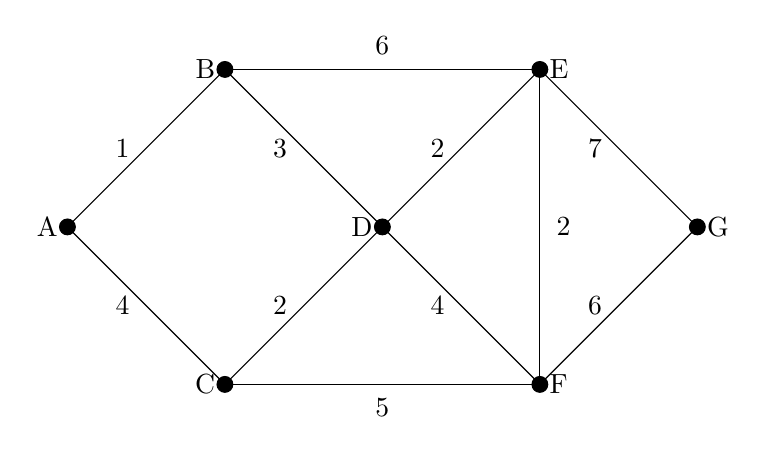
\begin{tikzpicture}
\draw[fill] (0,0) circle[radius=.1] node[left]{A};
\draw[fill] (2,2) circle[radius=.1] node[left]{B};
\draw[fill] (2,-2) circle[radius=.1] node[left]{C};
\draw[fill] (4,0) circle[radius=.1] node[left]{D};
\draw[fill] (6,2) circle[radius=.1] node[right]{E};
\draw[fill] (6,-2) circle[radius=.1] node[right]{F};
\draw[fill] (8,0) circle[radius=.1] node[right]{G};
\draw(0,0)--(2,2);
\node at (0.7,1){1};
\draw(0,0)--(2,-2);
\node at (0.7,-1){4};
\draw(2,2)--(4,0);
\node at (2.7,1){3};
\draw(2,-2)--(4,0);
\node at (2.7,-1){2};
\draw(4,0)--(6,2);
\node at (4.7,1){2};
\draw(4,0)--(6,-2);
\node at (4.7,-1){4};
\draw(6,2)--(8,0);
\node at (6.7,1){7};
\draw(6,-2)--(8,0);
\node at (6.7,-1){6};
\draw(2,2)--(6,2);
\node at (4,2.3){6};
\draw(2,-2)--(6,-2);
\node at (4,-2.3){5};
\draw(6,2)--(6,-2);
\node at (6.3,0){2};
\end{tikzpicture}
\end{exercise}


\section{Euler Circuits and the Chinese Postman Problem}
In the first section, we created a graph of the K\"onigsberg bridges and asked whether it was possible to walk across every bridge once.  Because Euler first studied this question, these types of paths are named after him.


\begin{definition}{Euler Path}{}
An \textbf{Euler path} is a path that uses every edge in a graph with no repeats.  Being a path, it does not have to return to the starting vertex.
\end{definition}

\begin{example}{}{}%5
In the graph shown below, there are several Euler paths.  One such path is CABDCB.  The path is shown in arrows to the right, with the order of edges numbered.\\
\begin{minipage}{.5\textwidth}
\begin{center}
\scalebox{.8}{
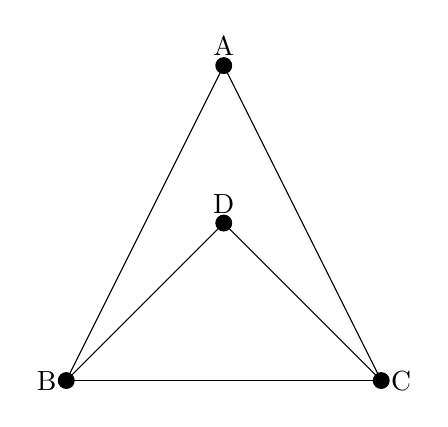
\begin{tikzpicture}
\draw[fill] (0,0) circle[radius=.1] node [left]{B};
\draw[fill] (4,0) circle[radius=.1] node [right]{C};
\draw[fill] (2,2) circle[radius=.1] node [above]{D};
\draw[fill] (2,4) circle[radius=.1] node [above]{A};
\draw(0,0)--(4,0);
\draw(0,0)--(2,2);
\draw(0,0)--(2,4);
\draw(4,0)--(2,2);
\draw(4,0)--(2,4);
\end{tikzpicture}
}
\end{center}
\end{minipage}
%
\begin{minipage}{.5\textwidth}
\begin{center}
\scalebox{0.8}{
\begin{tikzpicture}
\draw[fill] (0,0) circle[radius=.1] node [left]{B};
\draw[fill] (4,0) circle[radius=.1] node [right]{C};
\draw[fill] (2,2) circle[radius=.1] node [above]{D};
\draw[fill] (2,4) circle[radius=.1] node [above]{A};
\draw[directed](4,0)--(0,0);
\draw[directed](0,0)--(2,2);
\draw[directed] (2,4)--(0,0);
\draw[directed](2,2)--(4,0);
\draw[directed] (4,0)--(2,4);
\node at (2,-0.3){5};
\node at (1.4,1){3};
\node at (0.7,2.2){2};
\node at (2.7,1){4};
\node at (3.3,2.2){1};
\end{tikzpicture}
}
\end{center}
\end{minipage}
\end{example}

\begin{definition}{Euler Circuit}{}
An \textbf{Euler circuit} is a circuit that uses every edge in a graph with no repeats.  Being a circuit, it must start and end at the same vertex.
\end{definition}


\begin{example}{}{}%6
The graph below has several possible Euler circuits.  Here?s a couple, starting and ending at vertex A:  ADEACEFCBA and AECABCFEDA.  The second is shown in arrows.\\
\begin{minipage}{.5\textwidth}
\begin{center}
\scalebox{0.8}{
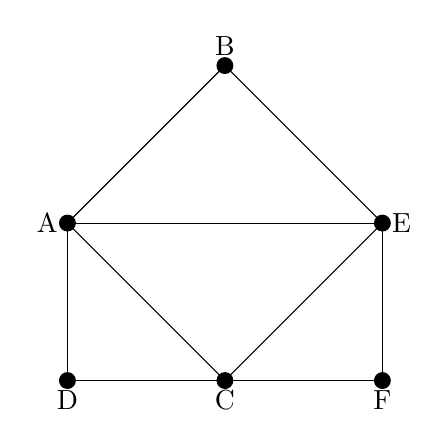
\begin{tikzpicture}
\draw[fill] (0,0) circle[radius=.1] node [below]{D};
\draw[fill] (0,2) circle[radius=.1] node [left]{A};
\draw[fill] (2,0) circle[radius=.1] node [below]{C};
\draw[fill] (4,0) circle[radius=.1] node [below]{F};
\draw[fill] (4,2) circle[radius=.1] node [right]{E};
\draw[fill] (2,4) circle[radius=.1] node [above]{B};
\draw(0,0)--(2,0);
\draw(0,0)--(0,2);
\draw(2,0)--(0,2);
\draw(2,0)--(4,2);
\draw(2,0)--(4,0);
\draw(0,2)--(4,2);
\draw(0,2)--(2,4);
\draw(2,4)--(4,2);
\draw(4,0)--(4,2);
\end{tikzpicture}
}
\end{center}
\end{minipage}
%
\begin{minipage}{.5\textwidth}
\begin{center}
\scalebox{0.8}{
\begin{tikzpicture}
\draw[fill] (0,0) circle[radius=.1] node [below]{B};
\draw[fill] (0,2) circle[radius=.1] node [left]{A};
\draw[fill] (2,0) circle[radius=.1] node [below]{C};
\draw[fill] (4,0) circle[radius=.1] node [below]{F};
\draw[fill] (4,2) circle[radius=.1] node [right]{E};
\draw[fill] (2,4) circle[radius=.1] node [above]{D};
\draw[directed](0,0)--(2,0);
\draw[directed](0,2)--(0,0);
\draw[directed](2,0)--(0,2);
\draw[directed](4,2)--(2,0);
\draw[directed](2,0)--(4,0);
\draw[directed](0,2)--(4,2);
\draw[directed](2,4)--(0,2);
\draw[directed](4,2)--(2,4);
\draw[directed](4,0)--(4,2);
\node at (-.3,1){4};
\node at (1,0.3){5};
\node at (1.3,1){3};
\node at (0.7,3){9};
\node at (2,2.3){1};
\node at (3.3,3){8};
\node at (2.6,1){2};
\node at (3,0.3){6};
\node at (4.3,1){7};
\end{tikzpicture}
}
\end{center}
\end{minipage}
\end{example}




Look back at the example used for Euler paths -- does that graph have an Euler circuit?  A few tries will tell you no; that graph does not have an Euler circuit.  When we were working with shortest paths, we were interested in the optimal path.  With Euler paths and circuits, we?re primarily interested in whether an Euler path or circuit \textit{exists}.  

Why do we care if an Euler circuit exists?  Think back to our housing development lawn inspector from the beginning of the chapter.  The lawn inspector is interested in walking as little as possible.  The ideal situation would be a circuit that covers every street with no repeats.  That's an Euler circuit!  Luckily, Euler solved the question of whether or not an Euler path or circuit will exist.


\begin{theorem}{Euler's Path and Circuit Theorems}{}
\hspace{3in}
\begin{itemize}
\item A graph will contain an Euler path if it contains at most two vertices of odd degree.
\item A graph will contain an Euler circuit if all vertices have even degree
\end{itemize}
\end{theorem}

\begin{example}{}{}%7
In the graph below, vertices A and C have degree 4, since there are 4 edges leading into each vertex.  B is degree 2, D is degree 3, and E is degree 1.  This graph contains two vertices with odd degree (D and E) and three vertices with even degree (A, B, and C), so Euler's theorems tell us this graph has an Euler path, but not an Euler circuit.\\
\scalebox{.8}{
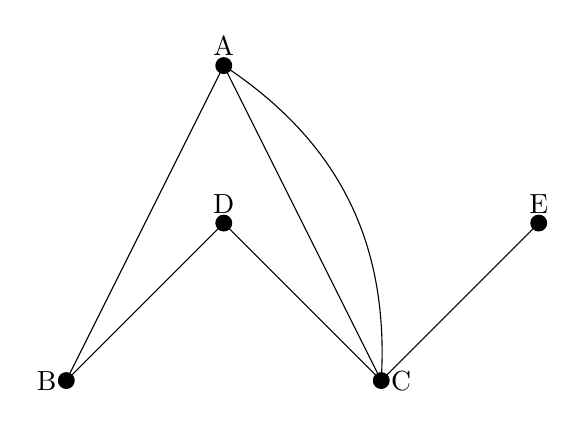
\begin{tikzpicture}
\draw[fill] (0,0) circle[radius=.1] node [left]{B};
\draw[fill] (4,0) circle[radius=.1] node [right]{C};
\draw[fill] (2,2) circle[radius=.1] node [above]{D};
\draw[fill] (2,4) circle[radius=.1] node [above]{A};
\draw[fill] (6,2) circle[radius=.1] node [above]{E};
\draw(4,0)--(6,2);
\draw(0,0)--(2,2);
\draw(0,0)--(2,4);
\draw(4,0)--(2,2);
\draw(4,0)--(2,4);
\draw (2,4) to [bend left] (4,0);
\end{tikzpicture}
}
\end{example}

\begin{example}%8
Is there an Euler circuit on the housing development lawn inspector graph we created earlier in the chapter?  All the highlighted vertices have odd degree.  Since there are more than two vertices with odd degree, there are no Euler paths or Euler circuits on this graph.  Unfortunately our lawn inspector will need to do some backtracking.

\begin{minipage}{0.5\textwidth}
\begin{tikzpicture}
    \foreach \pos/\name in {{(0,0)/A}, {(1,0)/D}, {(2,0)/G}, {(3,0)/N}, {(4,0)/O}, {(1,1)/B}, {(2,1)/E}, {(3,1)/F}, {(4,1)/M}, {(3,2)/C}, {(2,-1)/H}, {(3,-1)/J}, {(2,-2)/I}, {(3,-2)/K}, {(4,-2)/P}, {(5,-2)/Q}, {(3,-3)/L}, {(5,-3)/R}}
                \node[vertex] (\name) at \pos {$\name$};
                
 \foreach \source/ \dest in {A/D, D/G, A/B, B/E, B/C, C/F, E/F, F/M, D/E, E/G, G/H, H/I, H/J, I/K, J/K, K/L, N/J, F/N, F/M, N/O, O/P, P/Q, Q/R, M/O, K/P, L/R}
              \path (\source) edge (\dest);                
\end{tikzpicture}     
\end{minipage}
%
\begin{minipage}{0.5\textwidth}
\begin{tikzpicture}
    \foreach \pos/\name in {{(0,0)/A}, {(1,0)/D}, {(2,0)/G}, {(3,0)/N}, {(4,0)/O}, {(1,1)/B}, {(2,1)/E}, {(3,1)/F}, {(4,1)/M}, {(3,2)/C}, {(2,-1)/H}, {(3,-1)/J}, {(2,-2)/I}, {(3,-2)/K}, {(4,-2)/P}, {(5,-2)/Q}, {(3,-3)/L}, {(5,-3)/R}}
                \node[vertex] (\name) at \pos {$\name$};
                
 \foreach \source/ \dest in {A/D, D/G, A/B, B/E, B/C, C/F, E/F, F/M, D/E, E/G, G/H, H/I, H/J, I/K, J/K, K/L, N/J, F/N, F/M, N/O, O/P, P/Q, Q/R, M/O, K/P, L/R}
              \path (\source) edge (\dest); 
              
\draw[fill=yellow] (1,0) circle[radius=.3];
\node at (1,0){D};  
\draw[fill=yellow] (1,1) circle[radius=.3];
\node at (1,1){B};
\draw[fill=yellow] (2,0) circle[radius=.3];
\node at (2,0){G};   
\draw[fill=yellow] (3,0) circle[radius=.3];
\node at (3,0){N};
\draw[fill=yellow] (4,0) circle[radius=.3];
\node at (4,0){O};    
\draw[fill=yellow] (2,-1) circle[radius=.3];
\node at (2,-1){H};  
\draw[fill=yellow] (3,-1) circle[radius=.3];
\node at (3,-1){J}; 
\draw[fill=yellow] (4,-2) circle[radius=.3];
\node at (4,-2){P};                               
\end{tikzpicture}     
\end{minipage}
\end{example}



\begin{example}{}{}%9
When it snows in the same housing development, the snowplow has to plow both sides of every street.  For simplicity, we'll assume the plow is out early enough that it can ignore traffic laws and drive down either side of the street in either direction.  This can be visualized in the graph by drawing two edges for each street, representing the two sides of the street.\\

\begin{tikzpicture}
    \foreach \pos/\name in {{(0,0)/A}, {(1,0)/D}, {(2,0)/G}, {(3,0)/N}, {(4,0)/O}, {(1,1)/B}, {(2,1)/E}, {(3,1)/F}, {(4,1)/M}, {(3,2)/C}, {(2,-1)/H}, {(3,-1)/J}, {(2,-2)/I}, {(3,-2)/K}, {(4,-2)/P}, {(5,-2)/Q}, {(3,-3)/L}, {(5,-3)/R}}
                \node[vertex] (\name) at \pos {$\name$};
                
 \foreach \source/ \dest in {A/D, D/G, A/B, B/E, B/C, C/F, E/F, F/M, D/E, E/G, G/H, H/I, H/J, I/K, J/K, K/L, N/J, F/N, F/M, N/O, O/P, P/Q, Q/R, M/O, K/P, L/R}
              \path (\source) edge (\dest); 
           
   \foreach \source/ \dest in {A/D, D/G, A/B, B/E, B/C, C/F, E/F, F/M, D/E, E/G, G/H, H/I, H/J, I/K, J/K, K/L, N/J, F/N, F/M, N/O, O/P, P/Q, Q/R, M/O, K/P, L/R}
              \path (\source) edge[bend left] (\dest);             
 \end{tikzpicture}


Notice that every vertex in this graph has even degree, so this graph does have an Euler circuit.  
\end{example}

Now we know how to determine if a graph has an Euler circuit, but if it does, how do we find one?  While it usually is possible to find an Euler circuit just by pulling out your pencil and trying to find one, the more formal method is Fleury's algorithm.


\begin{algorithm}{}{}[Fleury's Algorithm]
\hspace{3in}
\begin{enumerate}
\item	Start at any vertex if finding an Euler circuit.  If finding an Euler path, start at one of the two vertices with odd degree.
\item	Choose any edge leaving your current vertex, provided deleting that edge will not separate the graph into two disconnected sets of edges.
\item	Add that edge to your circuit, and delete it from the graph.
\item	Continue until you're done.
\end{enumerate}
\end{algorithm}

\begin{example}{}{}%10
Let's find an Euler Circuit on this graph using Fleury's algorithm, starting at vertex A.\\

\begin{tabular}{|l|l|l|}
\hline
Original Graph. & AD deleted. D is current. & E is current.\\
Choosing edge AD. & Can't choose DC since that & From here, there is only one\\
&would disconnect the graph. &option, so the rest of the\\
&Choosing DE. &circuit is determined.\\
\hline
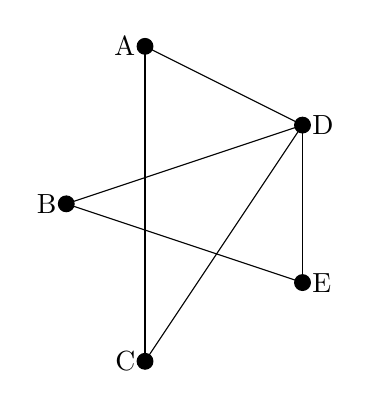
\begin{tikzpicture}
\draw[fill] (0,0) circle[radius=.1] node [left]{B};
\draw[fill] (1,2) circle[radius=.1] node [left]{A};
\draw[fill] (1,-2) circle[radius=.1] node [left]{C};
\draw[fill] (3,-1) circle[radius=.1] node [right]{E};
\draw[fill] (3,1) circle[radius=.1] node [right]{D};
\draw(0,0)--(3,1);
\draw(0,0)--(3,-1);
\draw(1,2)--(1,-2);
\draw(1,2)--(3,1);
\draw(1,-2)--(3,1);
\draw(3,1)--(3,-1);
\end{tikzpicture}
&
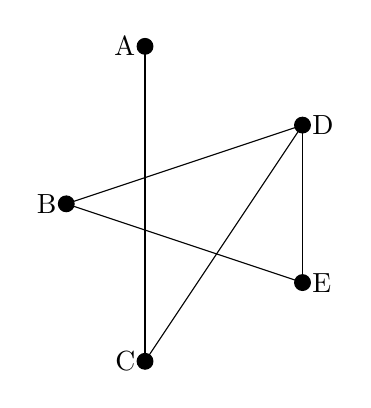
\begin{tikzpicture}
\draw[fill] (0,0) circle[radius=.1] node [left]{B};
\draw[fill] (1,2) circle[radius=.1] node [left]{A};
\draw[fill] (1,-2) circle[radius=.1] node [left]{C};
\draw[fill] (3,-1) circle[radius=.1] node [right]{E};
\draw[fill] (3,1) circle[radius=.1] node [right]{D};
\draw(0,0)--(3,1);
\draw(0,0)--(3,-1);
\draw(1,2)--(1,-2);
\draw(1,-2)--(3,1);
\draw(3,1)--(3,-1);
\end{tikzpicture}
&
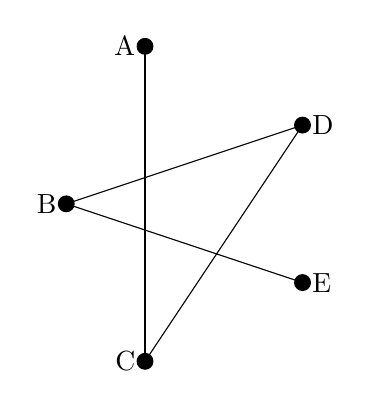
\begin{tikzpicture}
\draw[fill] (0,0) circle[radius=.1] node [left]{B};
\draw[fill] (1,2) circle[radius=.1] node [left]{A};
\draw[fill] (1,-2) circle[radius=.1] node [left]{C};
\draw[fill] (3,-1) circle[radius=.1] node [right]{E};
\draw[fill] (3,1) circle[radius=.1] node [right]{D};
\draw(0,0)--(3,1);
\draw(0,0)--(3,-1);
\draw(1,2)--(1,-2);
\draw(1,-2)--(3,1);
\end{tikzpicture}\\
Circuit so far: AD & Circuit so far: ADE & Circuit: ADEBDCA\\
\hline
\end{tabular}

\end{example}

\begin{exercise}{}{}%3
Does the graph below have an Euler Circuit?  If so, find one.\\

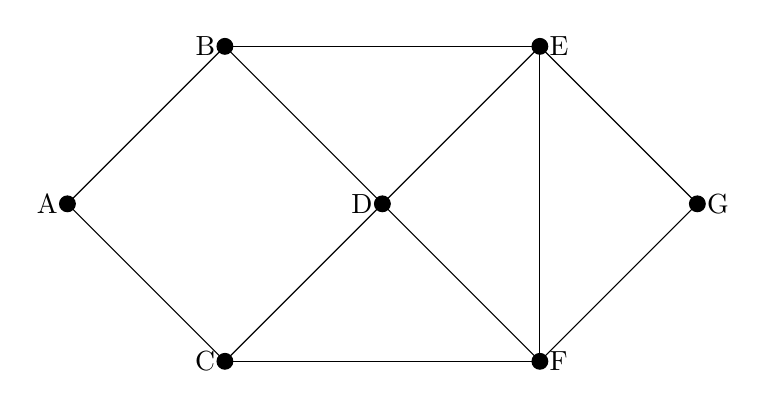
\begin{tikzpicture}
\draw[fill] (0,0) circle[radius=.1] node[left]{A};
\draw[fill] (2,2) circle[radius=.1] node[left]{B};
\draw[fill] (2,-2) circle[radius=.1] node[left]{C};
\draw[fill] (4,0) circle[radius=.1] node[left]{D};
\draw[fill] (6,2) circle[radius=.1] node[right]{E};
\draw[fill] (6,-2) circle[radius=.1] node[right]{F};
\draw[fill] (8,0) circle[radius=.1] node[right]{G};
\draw(0,0)--(2,2);
\draw(0,0)--(2,-2);
\draw(2,2)--(4,0);
\draw(2,-2)--(4,0);
\draw(4,0)--(6,2);
\draw(4,0)--(6,-2);
\draw(6,2)--(8,0);
\draw(6,-2)--(8,0);
\draw(2,2)--(6,2);
\draw(2,-2)--(6,-2);
\draw(6,2)--(6,-2);
\end{tikzpicture}
\end{exercise}


\subsection{Eulerization and the Chinese Postman Problem}
Not every graph has an Euler path or circuit, yet our lawn inspector still needs to do her inspections.  Her goal is to minimize the amount of walking she has to do.  In order to do that, she will have to duplicate some edges in the graph until an Euler circuit exists. 

\begin{definition}{Eulerization}{}[]
\textbf{Eulerization} is the process of adding edges to a graph to create an Euler circuit on a graph.  To eulerize a graph, edges are duplicated to connect pairs of vertices with odd degree.  Connecting two odd degree vertices increases the degree of each, giving them both even degree.  When two odd degree vertices are not directly connected, we can duplicate all edges in a path connecting the two.
\end{definition}

Note that we can only duplicate edges, not create edges where there wasn't one before.  Duplicating edges would mean walking or driving down a road twice, while creating an edge where there wasn't one before is akin to installing a new road!


\begin{example}{}{} %11
For the rectangular graph shown, three possible eulerizations are shown.  Notice in each of these cases the vertices that started with odd degrees have even degrees after eulerization, allowing for an Euler circuit.\\

\begin{center}
\begin{tabular}{p{5cm} p{5cm}}
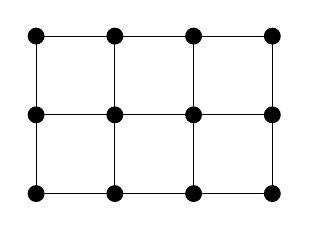
\begin{tikzpicture}
\draw[fill] (0,2) circle[radius=.1];
\draw[fill] (1,2) circle[radius=.1];
\draw[fill] (2,2) circle[radius=.1];
\draw[fill] (3,2) circle[radius=.1];
\draw[fill] (0,1) circle[radius=.1];
\draw[fill] (1,1) circle[radius=.1];
\draw[fill] (2,1) circle[radius=.1]; 
\draw[fill] (3,1) circle[radius=.1];
\draw[fill] (0,0) circle[radius=.1];
\draw[fill] (1,0) circle[radius=.1];
\draw[fill] (2,0) circle[radius=.1];
\draw[fill] (3,0) circle[radius=.1];
\draw(0,0)--(0,1);
\draw(0,1)--(0,2);
\draw(1,0)--(1,1);
\draw(1,1)--(1,2);
\draw(2,0)--(2,1);
\draw(2,1)--(2,2);
\draw(3,0)--(3,1);
\draw(3,1)--(3,2);
\draw(0,0)--(1,0);
\draw(1,0)--(2,0);
\draw(2,0)--(3,0);
\draw(0,1)--(1,1);
\draw(1,1)--(2,1);
\draw(2,1)--(3,1);
\draw(0,2)--(1,2);
\draw(1,2)--(2,2);
\draw(2,2)--(3,2);
\end{tikzpicture}
&
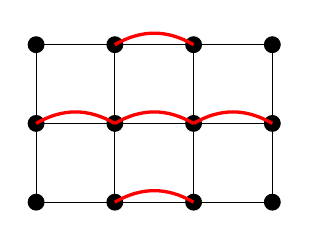
\begin{tikzpicture}
\draw[fill] (0,2) circle[radius=.1];
\draw[fill] (1,2) circle[radius=.1];
\draw[fill] (2,2) circle[radius=.1];
\draw[fill] (3,2) circle[radius=.1];
\draw[fill] (0,1) circle[radius=.1];
\draw[fill] (1,1) circle[radius=.1];
\draw[fill] (2,1) circle[radius=.1]; 
\draw[fill] (3,1) circle[radius=.1];
\draw[fill] (0,0) circle[radius=.1];
\draw[fill] (1,0) circle[radius=.1];
\draw[fill] (2,0) circle[radius=.1];
\draw[fill] (3,0) circle[radius=.1];
\draw(0,0)--(0,1);
\draw(0,1)--(0,2);
\draw(1,0)--(1,1);
\draw(1,1)--(1,2);
\draw(2,0)--(2,1);
\draw(2,1)--(2,2);
\draw(3,0)--(3,1);
\draw(3,1)--(3,2);
\draw(0,0)--(1,0);
\draw(1,0)--(2,0);
\draw(2,0)--(3,0);
\draw(0,1)--(1,1);
\draw(1,1)--(2,1);
\draw(2,1)--(3,1);
\draw(0,2)--(1,2);
\draw(1,2)--(2,2);
\draw(2,2)--(3,2);
\draw[very thick, red] (1,2) to [bend left] (2,2);
\draw[very thick, red] (0,1) to [bend left] (1,1);
\draw[very thick, red] (1,1) to [bend left] (2,1);
\draw[very thick, red] (2,1) to [bend left] (3,1);
\draw[very thick, red] (1,0) to [bend left] (2,0);
\end{tikzpicture}\\
&\\
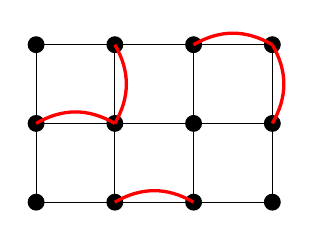
\begin{tikzpicture}
\draw[fill] (0,2) circle[radius=.1];
\draw[fill] (1,2) circle[radius=.1];
\draw[fill] (2,2) circle[radius=.1];
\draw[fill] (3,2) circle[radius=.1];
\draw[fill] (0,1) circle[radius=.1];
\draw[fill] (1,1) circle[radius=.1];
\draw[fill] (2,1) circle[radius=.1]; 
\draw[fill] (3,1) circle[radius=.1];
\draw[fill] (0,0) circle[radius=.1];
\draw[fill] (1,0) circle[radius=.1];
\draw[fill] (2,0) circle[radius=.1];
\draw[fill] (3,0) circle[radius=.1];
\draw(0,0)--(0,1);
\draw(0,1)--(0,2);
\draw(1,0)--(1,1);
\draw(1,1)--(1,2);
\draw(2,0)--(2,1);
\draw(2,1)--(2,2);
\draw(3,0)--(3,1);
\draw(3,1)--(3,2);
\draw(0,0)--(1,0);
\draw(1,0)--(2,0);
\draw(2,0)--(3,0);
\draw(0,1)--(1,1);
\draw(1,1)--(2,1);
\draw(2,1)--(3,1);
\draw(0,2)--(1,2);
\draw(1,2)--(2,2);
\draw(2,2)--(3,2);
\draw[very thick, red] (2,2) to [bend left] (3,2);
\draw[very thick, red] (0,1) to [bend left] (1,1);
\draw[very thick, red] (1,0) to [bend left] (2,0);
\draw[very thick, red] (1,2) to [bend left] (1,1);
\draw[very thick, red] (3,2) to [bend left] (3,1);
\end{tikzpicture}
&
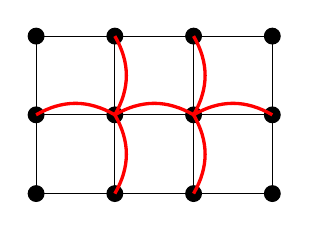
\begin{tikzpicture}
\draw[fill] (0,2) circle[radius=.1];
\draw[fill] (1,2) circle[radius=.1];
\draw[fill] (2,2) circle[radius=.1];
\draw[fill] (3,2) circle[radius=.1];
\draw[fill] (0,1) circle[radius=.1];
\draw[fill] (1,1) circle[radius=.1];
\draw[fill] (2,1) circle[radius=.1]; 
\draw[fill] (3,1) circle[radius=.1];
\draw[fill] (0,0) circle[radius=.1];
\draw[fill] (1,0) circle[radius=.1];
\draw[fill] (2,0) circle[radius=.1];
\draw[fill] (3,0) circle[radius=.1];
\draw(0,0)--(0,1);
\draw(0,1)--(0,2);
\draw(1,0)--(1,1);
\draw(1,1)--(1,2);
\draw(2,0)--(2,1);
\draw(2,1)--(2,2);
\draw(3,0)--(3,1);
\draw(3,1)--(3,2);
\draw(0,0)--(1,0);
\draw(1,0)--(2,0);
\draw(2,0)--(3,0);
\draw(0,1)--(1,1);
\draw(1,1)--(2,1);
\draw(2,1)--(3,1);
\draw(0,2)--(1,2);
\draw(1,2)--(2,2);
\draw(2,2)--(3,2);
\draw[very thick, red] (0,1) to [bend left] (1,1);
\draw[very thick, red] (1,1) to [bend left] (2,1);
\draw[very thick, red] (2,1) to [bend left] (3,1);
\draw[very thick, red] (1,2) to [bend left] (1,1);
\draw[very thick, red] (1,1) to [bend left] (1,0);
\draw[very thick, red] (2,2) to [bend left] (2,1);
\draw[very thick, red] (2,1) to [bend left] (2,0);
\end{tikzpicture}\\
\end{tabular}
\end{center}
\end{example}



In the example above, you'll notice that the last eulerization required duplicating seven edges, while the first two only required duplicating five edges.  If we were eulerizing the graph to find a walking path, we would want the eulerization with minimal duplications.  If the edges had weights representing distances or costs, then we would want to select the eulerization with the minimal total added weight.


\begin{exercise}{}{} %4
Eulerize the graph shown, then find an Euler circuit on the eulerized graph.\\
\scalebox{.8}{
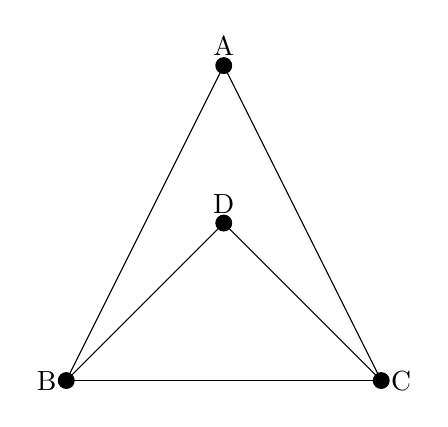
\begin{tikzpicture}
\draw[fill] (0,0) circle[radius=.1] node [left]{B};
\draw[fill] (4,0) circle[radius=.1] node [right]{C};
\draw[fill] (2,2) circle[radius=.1] node [above]{D};
\draw[fill] (2,4) circle[radius=.1] node [above]{A};
\draw(0,0)--(4,0);
\draw(0,0)--(2,2);
\draw(0,0)--(2,4);
\draw(4,0)--(2,2);
\draw(4,0)--(2,4);
\end{tikzpicture}
}
\end{exercise}


\begin{example}{}{}% 12
Looking again at the graph for our lawn inspector from Examples 1 and 8, the vertices with odd degree are shown highlighted.  With eight vertices, we will always have to duplicate at least four edges.  In this case, we need to duplicate five edges since two odd degree vertices are not directly connected.  Without weights we can?t be certain this is the eulerization that minimizes walking distance, but it looks pretty good.

\textcolor{red}{PICTURE from above}
\end{example}


The problem of finding the optimal eulerization is called the Chinese Postman Problem, a name given by an American in honor of the Chinese mathematician Mei-Ko Kwan who first studied the problem in 1962 while trying to find optimal delivery routes for postal carriers.   This problem is important in determining efficient routes for garbage trucks, school buses, parking meter checkers, street sweepers, and more.

Unfortunately, algorithms to solve this problem are fairly complex.  Some simpler cases are considered in the exercises.

\section{Hamiltonian Circuits and the Traveling Salesman Problem}
In the last section, we considered optimizing a walking route for a postal carrier.  How is this different than the requirements of a package delivery driver?  While the postal carrier needed to walk down every street (edge) to deliver the mail, the package delivery driver instead needs to visit every one of a set of delivery locations.  Instead of looking for a circuit that covers every edge once, the package deliverer is interested in a circuit that visits every vertex once.


\begin{definition}{Hamiltonian Circuits and Paths}{}[]
A Hamiltonian circuit is a circuit that visits every vertex once with no repeats.  Being a circuit, it must start and end at the same vertex.  A Hamiltonian path also visits every vertex once with no repeats, but does not have to start and end at the same vertex.  
\end{definition}


Hamiltonian circuits are named for William Rowan Hamilton who studied them in the 1800?s.

\begin{example}{}{} % 13
One Hamiltonian circuit is shown on the graph below.  There are several other Hamiltonian circuits possible on this graph.  Notice that the circuit only has to visit every vertex once; it does not need to use every edge.  

This circuit could be notated by the sequence of vertices visited, starting and ending at the same vertex: ABFGCDHMLKJEA.  Notice that the same circuit could be written in reverse order, or starting and ending at a different vertex.
\begin{center}
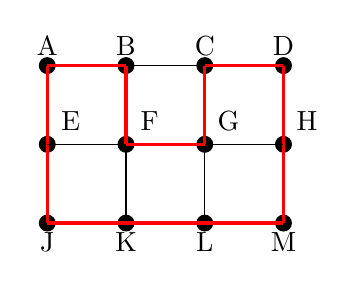
\begin{tikzpicture}
\draw[fill] (0,2) circle[radius=.1] node[above]{A};
\draw[fill] (1,2) circle[radius=.1] node[above]{B};
\draw[fill] (2,2) circle[radius=.1] node[above]{C};
\draw[fill] (3,2) circle[radius=.1] node[above]{D};
\draw[fill] (0,1) circle[radius=.1];
\node at (0.3,1.3){E}; 
\draw[fill] (1,1) circle[radius=.1];
\node at (1.3,1.3){F}; 
\draw[fill] (2,1) circle[radius=.1];
\node at (2.3,1.3){G};  
\draw[fill] (3,1) circle[radius=.1];
\node at (3.3,1.3){H};  
\draw[fill] (0,0) circle[radius=.1] node[below]{J};
\draw[fill] (1,0) circle[radius=.1] node[below]{K};
\draw[fill] (2,0) circle[radius=.1] node[below]{L};
\draw[fill] (3,0) circle[radius=.1] node[below]{M};
\draw[very thick, red](0,0)--(0,1);
\draw[very thick, red](0,1)--(0,2);
\draw(1,0)--(1,1);
\draw[very thick, red](1,1)--(1,2);
\draw(2,0)--(2,1);
\draw[very thick, red](2,1)--(2,2);
\draw[very thick, red](3,0)--(3,1);
\draw[very thick, red](3,1)--(3,2);
\draw[very thick, red](0,0)--(1,0);
\draw[very thick, red](1,0)--(2,0);
\draw[very thick, red](2,0)--(3,0);
\draw(0,1)--(1,1);
\draw[very thick, red](1,1)--(2,1);
\draw(2,1)--(3,1);
\draw[very thick, red](0,2)--(1,2);
\draw(1,2)--(2,2);
\draw[very thick, red](2,2)--(3,2);
\end{tikzpicture}
\end{center}
\end{example}


Unlike with Euler circuits, there is no nice theorem that allows us to instantly determine whether or not a Hamiltonian circuit exists for all graphs\footnote{There are some theorems that can be used in specific circumstances, such as Dirac's theorem, which says that a Hamilton circuit must exist on a graph with $n$ vertices if each vertex has degree $\frac{n}{2}$ or greater.}.  

\begin{example}{}{} %14
Does a Hamiltonian path or circuit exist on the graph below?\\

\scalebox{.8}{
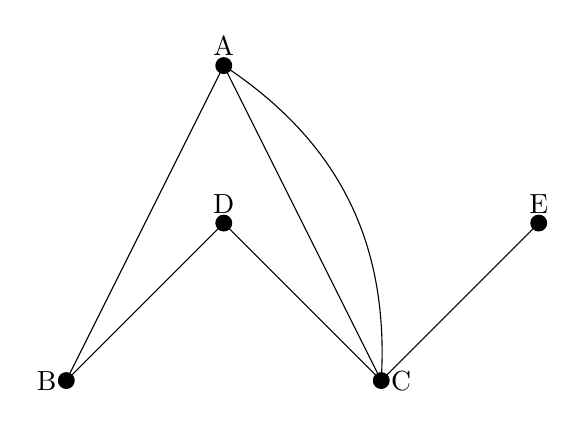
\begin{tikzpicture}
\draw[fill] (0,0) circle[radius=.1] node [left]{B};
\draw[fill] (4,0) circle[radius=.1] node [right]{C};
\draw[fill] (2,2) circle[radius=.1] node [above]{D};
\draw[fill] (2,4) circle[radius=.1] node [above]{A};
\draw[fill] (6,2) circle[radius=.1] node [above]{E};
\draw(4,0)--(6,2);
\draw(0,0)--(2,2);
\draw(0,0)--(2,4);
\draw(4,0)--(2,2);
\draw(4,0)--(2,4);
\draw (2,4) to [bend left] (4,0);
\end{tikzpicture}
}

We can see that once we travel to vertex E there is no way to leave without returning to C, so there is no possibility of a Hamiltonian circuit.  If we start at vertex E we can find several Hamiltonian paths, such as ECDAB and ECABD.
\end{example}

With Hamiltonian circuits, our focus will not be on existence, but on the question of optimization; given a graph where the edges have weights, can we find the optimal Hamiltonian circuit; the one with lowest total weight.\\
\begin{minipage}{0.5\textwidth}
This problem is called the \textbf{Traveling salesman problem} (TSP) because the question can be framed like this:  Suppose a salesman needs to give sales pitches in four cities.  He looks up the airfares between each city, and puts the costs in a graph.  In what order should he travel to visit each city once then return home with the lowest cost? 
\end{minipage}
%
\begin{minipage}{0.5\textwidth}
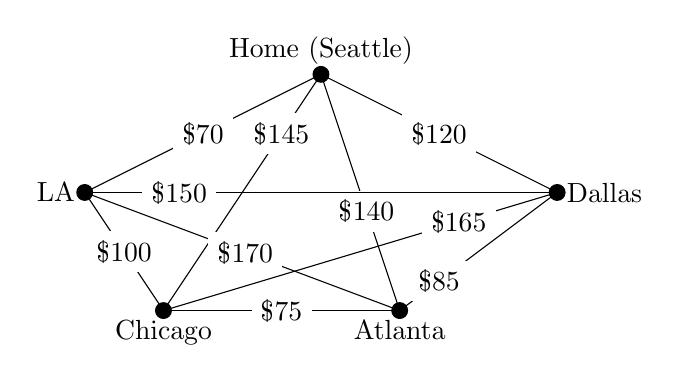
\begin{tikzpicture}
\draw[fill] (0,0) circle[radius=.1] node[below]{Chicago};
\draw[fill] (3,0) circle[radius=.1] node[below]{Atlanta};
\draw[fill] (-1,1.5) circle[radius=.1] node[left]{LA};
\draw[fill] (2,3) circle[radius=.1] node[above]{Home (Seattle)};
\draw[fill] (5,1.5) circle[radius=.1] node[right]{Dallas};
\draw(0,0)  to node[fill=white]{\$75}(3,0);
\draw(0,0)  to node[near end, fill=white]{\$145}(2,3);
\draw(0,0)  to node[fill=white]{\$100}(-1,1.5);
\draw(0,0)  to node[near end, fill=white]{\$165}(5,1.5);
\draw(3,0)  to node[pos=0.49,fill=white]{\$170}(-1,1.5);
\draw(3,0)  to node[pos=0.42, fill=white]{\$140}(2,3);
\draw(3,0) to node[near start, fill=white]{\$85}(5,1.5);
\draw(-1,1.5) to node[fill=white]{\$70}(2,3);
\draw(-1,1.5)  to node[pos=0.2, fill=white]{\$150}(5,1.5);
\draw(2,3)  to node[fill=white]{\$120}(5,1.5);
\end{tikzpicture}
\end{minipage}

To answer this question of how to find the lowest cost Hamiltonian circuit, we will consider some possible approaches.  The first option that might come to mind is to just try all different possible circuits.

\begin{algorithm}{}{}[Brute Force Algorithm (a.k.a. exhaustive search)]
\hspace{3in}
\begin{enumerate}
\item	List all possible Hamiltonian circuits
\item	Find the length of each circuit by adding the edge weights
\item	Select the circuit with minimal total weight.
\end{enumerate}
\end{algorithm}

\begin{example}{}{} %15
Apply the Brute force algorithm to find the minimum cost Hamiltonian circuit on the graph below.\\

\begin{center}
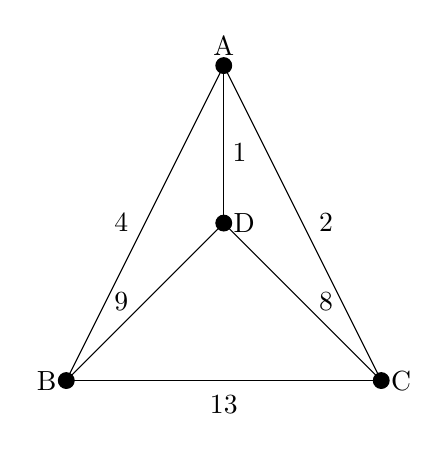
\begin{tikzpicture}
\draw[fill] (0,0) circle[radius=.1] node [left]{B};
\draw[fill] (4,0) circle[radius=.1] node [right]{C};
\draw[fill] (2,2) circle[radius=.1] node [right]{D};
\draw[fill] (2,4) circle[radius=.1] node [above]{A};
\draw(0,0)--(4,0);
\draw(0,0)--(2,2);
\draw(0,0)--(2,4);
\draw(4,0)--(2,2);
\draw(4,0)--(2,4);
\draw(2,4)--(2,2);
\node at (2,-0.3){13};
\node at (0.7,1){9};
\node at (0.7,2){4};
\node at (3.3,1){8};
\node at (3.3,2){2};
\node at (2.2,2.9){1};
\end{tikzpicture}
\end{center}

To apply the Brute force algorithm, we list all possible Hamiltonian circuits and calculate their weight:
\begin{center}
\begin{tabular}{|l|l|}
\hline
Circuit & Weight\\
\hline 
ABCDA & $4+13+8+1=26$\\
\hline
ABDCA & $4+9+8+2=23$\\
\hline
ACBDA & $2+13+9+1=25$\\
\hline
\end{tabular}
\end{center}

Note:  These are the unique circuits on this graph.  All other possible circuits are the reverse of the listed ones or start at a different vertex, but result in the same weights.

From this we can see that the second circuit, ABDCA, is the optimal circuit.  
\end{example}

The Brute force algorithm is optimal; it will always produce the Hamiltonian circuit with minimum weight.  Is it efficient?  To answer that question, we need to consider how many Hamiltonian circuits a graph could have.  For simplicity, let's look at the worst-case possibility, where every vertex is connected to every other vertex.  This is called a \textbf{complete graph}.

Suppose we had a complete graph with five vertices like the air travel graph above.  From Seattle there are four cities we can visit first.  From each of those, there are three choices.  From each of those cities, there are two possible cities to visit next.  There is then only one choice for the last city before returning home.  

This can be shown visually:\\

\noindent \scalebox{.5}{
\begin{tikzpicture}
\node at (0,0){A};
\node at (1,0){C};
\node at (2.5,0){A};
\node at (3.5,0){D};
\node at (5,0){D};
\node at (6,0){C};

\node at (8,0){A};
\node at (9,0){C};
\node at (10.5,0){A};
\node at (11.5,0){L};
\node at (13,0){L};
\node at (14,0){C};

\node at (16,0){A};
\node at (17,0){L};
\node at (18.5,0){A};
\node at (19.5,0){D};
\node at (21,0){D};
\node at (22,0){L};

\node at (23,0){L};
\node at (24,0){C};
\node at (25.5,0){L};
\node at (26.5,0){D};
\node at (28,0){D};
\node at (29,0){C};

%%%

\node at (0,1){C};
\node at (1,1){A};
\node at (2.5,1){D};
\node at (3.5,1){A};
\node at (5,1){C};
\node at (6,1){D};

\node at (8,1){C};
\node at (9,1){A};
\node at (10.5,1){L};
\node at (11.5,1){A};
\node at (13,1){C};
\node at (14,1){L};

\node at (16,1){L};
\node at (17,1){A};
\node at (18.5,1){D};
\node at (19.5,1){A};
\node at (21,1){L};
\node at (22,1){D};

\node at (23,1){C};
\node at (24,1){L};
\node at (25.5,1){D};
\node at (26.5,1){L};
\node at (28,1){C};
\node at (29,1){D};

%%%% Edges

\draw[directed1](0,.8)--(0,.2);
\draw[directed1](1,.8)--(1,.2);
\draw[directed1](2.5,.8)--(2.5,.2);
\draw[directed1](3.5,.8)--(3.5,.2);
\draw[directed1](5,.8)--(5,.2);
\draw[directed1](6,.8)--(6,.2);

\draw[directed1](8,.8)--(8,.2);
\draw[directed1](9,.8)--(9,.2);
\draw[directed1](10.5,.8)--(10.5,.2);
\draw[directed1](11.5,.8)--(11.5,.2);
\draw[directed1](13,.8)--(13,.2);
\draw[directed1](14,.8)--(14,.2);

\draw[directed1](16,.8)--(16,.2);
\draw[directed1](17,.8)--(17,.2);
\draw[directed1](18.5,.8)--(18.5,.2);
\draw[directed1](19.5,.8)--(19.5,.2);
\draw[directed1](21,.8)--(21,.2);
\draw[directed1](22,.8)--(22,.2);

\draw[directed1](23,.8)--(23,.2);
\draw[directed1](24,.8)--(24,.2);
\draw[directed1](25.5,.8)--(25.5,.2);
\draw[directed1](26.5,.8)--(26.5,.2);
\draw[directed1](28,.8)--(28,.2);
\draw[directed1](29,.8)--(29,.2);
%%%%

\node at (0.5,2){D};
\node at (3,2){C};
\node at (5.5,2){A};

\node at (8.5,2){L};
\node at (11,2){C};
\node at (13.5,2){A};

\node at (16.5,2){D};
\node at (19,2){L};
\node at (21.5,2){A};

\node at (23.5,2){D};
\node at (26,2){C};
\node at (28.5,2){L};

%%%%% Edges

\draw[directed1](0.5,1.8)--(0,1.2);
\draw[directed1](0.5,1.8)--(1,1.2);
\draw[directed1](3,1.8)--(2.5,1.2);
\draw[directed1](3,1.8)--(3.5,1.2);
\draw[directed1](5.5,1.8)--(5,1.2);
\draw[directed1](5.5,1.8)--(6,1.2);

\draw[directed1](8.5,1.8)--(8,1.2);
\draw[directed1](8.5,1.8)--(9,1.2);
\draw[directed1](11,1.8)--(10.5,1.2);
\draw[directed1](11,1.8)--(11.5,1.2);
\draw[directed1](13.5,1.8)--(13,1.2);
\draw[directed1](13.5,1.8)--(14,1.2);

\draw[directed1](16.5,1.8)--(16,1.2);
\draw[directed1](16.5,1.8)--(17,1.2);
\draw[directed1](19,1.8)--(18.5,1.2);
\draw[directed1](19,1.8)--(19.5,1.2);
\draw[directed1](21.5,1.8)--(21,1.2);
\draw[directed1](21.5,1.8)--(22,1.2);

\draw[directed1](23.5,1.8)--(23,1.2);
\draw[directed1](23.5,1.8)--(24,1.2);
\draw[directed1](26,1.8)--(25.5,1.2);
\draw[directed1](26,1.8)--(26.5,1.2);
\draw[directed1](28.5,1.8)--(28,1.2);
\draw[directed1](28.5,1.8)--(29,1.2);


%%%%%%%%%%%%%%%

\node at (3,3){LA};

\node at (11,3){Dallas};

\node at (19,3){Chicago};

\node at (26,3){Atlanta};

%%%%% Edges
\draw[directed1](3,2.8)--(0.5,2.2);
\draw[directed1](3,2.8)--(3,2.2);
\draw[directed1](3,2.8)--(5.5,2.2);

\draw[directed1](11,2.8)--(8.5,2.2);
\draw[directed1](11,2.8)--(11,2.2);
\draw[directed1](11,2.8)--(13.5,2.2);

\draw[directed1](19,2.8)--(16.5,2.2);
\draw[directed1](19,2.8)--(19,2.2);
\draw[directed1](19,2.8)--(21.5,2.2);

\draw[directed1](26,2.8)--(23.5,2.2);
\draw[directed1](26,2.8)--(26,2.2);
\draw[directed1](26,2.8)--(28.5,2.2);

%%%%%%%%%%%
\node at (15,5){Home(Seattle)};
\draw[directed1](15,4.8)--(3,3.2);
\draw[directed1](15,4.8)--(11,3.2);
\draw[directed1](15,4.8)--(19,3.2);
\draw[directed1](15,4.8)--(26,3.2);
\end{tikzpicture}
}



\noindent Counting the number of routes, we can see there are $4\cdot 3\cdot 2 \cdot 1 = 24$ routes.  For six cities there would be $5\cdot 4\cdot 3\cdot 2 \cdot 1 =120$ routes.  


\begin{theorem}{Number of Possible Circuits}{}[]
\hspace{1in}\\
For $N$ vertices in a complete graph, there will be $(n-1)!=(n-1)(n-2)(n-3)\cdots 3\cdot 2\cdot 1$ routes.  Half of these are duplicates in reverse order, so there are $\frac{(n-1)!}{2}$ unique circuits.\\

\noindent The exclamation symbol, $!$,  is read ``factorial" and is shorthand for the product shown.
\end{theorem}

\begin{example}{}{} % 16
How many circuits would a complete graph with 8 vertices have?\\

A complete graph with 8 vertices would have $(8-1)!=7!=7\cdot 6 \cdot 5\cdot 4\cdot 3\cdot 2\cdot 1 = 5040$ possible Hamiltonian circuits.  Half of the circuits are duplicates of other circuits but in reverse order, leaving 2520 unique routes.  
\end{example}


While this is a lot, it doesn't seem unreasonably huge.  But consider what happens as the number of cities increase:
\begin{center}
\begin{tabular}{|l|l|}
\hline
Cities &Unique Hamiltonian Circuits\\
\hline
9&8!/2 = 20,160\\
\hline
10&9!/2 = 181,440\\
\hline
11&10!/2 = 1,814,400\\
\hline
15 &14!/2 = 43,589,145,600\\
\hline
20&19!/2 = 60,822,550,204,416,000\\
\hline
\end{tabular}
\end{center}

As you can see the number of circuits is growing extremely quickly.  If a computer looked at one billion circuits a second, it would still take almost two years to examine all the possible circuits with only 20 cities!  Certainly Brute Force is \underline{not} an efficient algorithm.  


Unfortunately, no one has yet found an efficient \textit{and} optimal algorithm to solve the TSP, and it is very unlikely anyone ever will.  Since it is not practical to use brute force to solve the problem, we turn instead to \textbf{heuristic algorithms}; efficient algorithms that give approximate solutions.  In other words, heuristic algorithms are fast, but may or may not produce the optimal circuit.

\begin{algorithm}{}{}[Nearest Neighbor Algorithm (NNA)]
\hspace{3in}
\begin{enumerate}
\item	Select a starting point.
\item	Move to the nearest unvisited vertex (the edge with smallest weight).
\item	Repeat until the circuit is complete.
\end{enumerate}
\end{algorithm}

\begin{example}\label{graph17_ex} %17
Consider our earlier graph, shown below.  

\begin{center}
\scalebox{.8}{
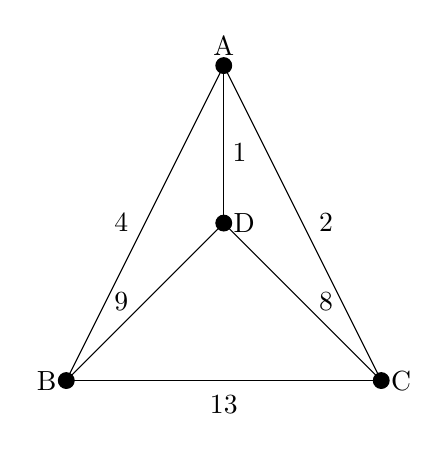
\begin{tikzpicture}
\draw[fill] (0,0) circle[radius=.1] node [left]{B};
\draw[fill] (4,0) circle[radius=.1] node [right]{C};
\draw[fill] (2,2) circle[radius=.1] node [right]{D};
\draw[fill] (2,4) circle[radius=.1] node [above]{A};
\draw(0,0)--(4,0);
\draw(0,0)--(2,2);
\draw(0,0)--(2,4);
\draw(4,0)--(2,2);
\draw(4,0)--(2,4);
\draw(2,4)--(2,2);
\node at (2,-0.3){13};
\node at (0.7,1){9};
\node at (0.7,2){4};
\node at (3.3,1){8};
\node at (3.3,2){2};
\node at (2.2,2.9){1};
\end{tikzpicture}
}
\end{center}
\noindent Starting at vertex A, the nearest neighbor is vertex D with a weight of 1.\\
From D, the nearest neighbor is C, with a weight of 8.  \\
From C, our only option is to move to vertex B, the only unvisited vertex, with a cost of 13.  \\
From B we return to A with a weight of 4.  \\

\noindent The resulting circuit is ADCBA with a total weight of $1+8+13+4 = 26$.
\end{example}

We ended up finding the worst circuit in the graph!  What happened?  Unfortunately, while it is very easy to implement, the NNA is a \textbf{greedy algorithm}, meaning it only looks at the immediate decision without considering the consequences in the future.  In this case, following the edge AD forced us to use the very expensive edge BC later.


\begin{example}{}{}%18
Consider again our salesman.  Starting in Seattle, the nearest neighbor (cheapest flight) is to LA, at a cost of \$70.  From there:

\begin{minipage}{0.5\textwidth}
\noindent LA to Chicago:  \$100\\
Chicago to Atlanta: \$75\\
Atlanta to Dallas: \$85\\
Dallas to Seattle: \$120\\
Total cost: \$450\\
\end{minipage}
%
\begin{minipage}{0.5\textwidth}
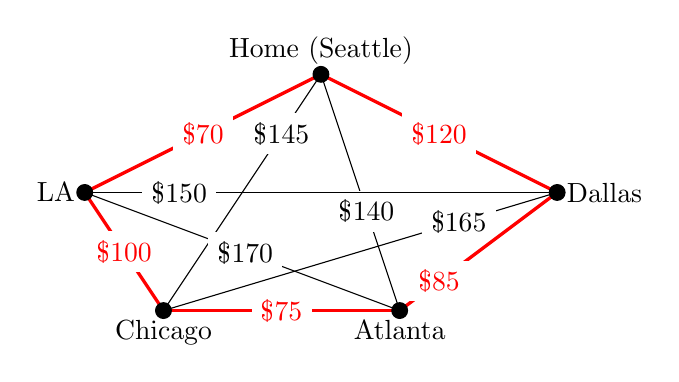
\begin{tikzpicture}
\draw[very thick, red](0,0)  to node[fill=white]{\$75}(3,0);
\draw(0,0)  to node[near end, fill=white]{\$145}(2,3);
\draw[very thick, red](0,0)  to node[fill=white]{\$100}(-1,1.5);
\draw(0,0)  to node[near end, fill=white]{\$165}(5,1.5);
\draw(3,0)  to node[pos=0.49,fill=white]{\$170}(-1,1.5);
\draw(3,0)  to node[pos=0.42, fill=white]{\$140}(2,3);
\draw[very thick, red](3,0) to node[near start, fill=white]{\$85}(5,1.5);
\draw[very thick, red](-1,1.5) to node[fill=white]{\$70}(2,3);
\draw(-1,1.5)  to node[pos=0.2, fill=white]{\$150}(5,1.5);
\draw[very thick, red](2,3)  to node[fill=white]{\$120}(5,1.5);
\draw[fill] (0,0) circle[radius=.1] node[below]{Chicago};
\draw[fill] (3,0) circle[radius=.1] node[below]{Atlanta};
\draw[fill] (-1,1.5) circle[radius=.1] node[left]{LA};
\draw[fill] (2,3) circle[radius=.1] node[above]{Home (Seattle)};
\draw[fill] (5,1.5) circle[radius=.1] node[right]{Dallas};
\end{tikzpicture}
\end{minipage}

\noindent In this case, nearest neighbor did find the optimal circuit.  
\end{example}


Going back to our first example, how could we improve the outcome?  One option would be to redo the nearest neighbor algorithm with a different starting point to see if the result changed.  Since nearest neighbor is so fast, doing it several times isn't a big deal.

\begin{algorithm}{}{}[Repeated Nearest Neighbor Algorithm (RNNA)]
\hspace{3in}
\begin{enumerate}
\item	Do the Nearest Neighbor Algorithm starting at each vertex
\item	Choose the circuit produced with minimal total weight
\end{enumerate}
\end{algorithm}

\begin{example}{}{} % 19
We will revisit the graph from Example~\ref{graph17_ex}.\\
\begin{center}
\scalebox{.8}{
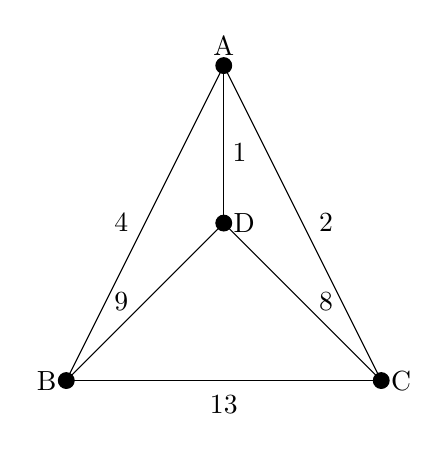
\begin{tikzpicture}
\draw[fill] (0,0) circle[radius=.1] node [left]{B};
\draw[fill] (4,0) circle[radius=.1] node [right]{C};
\draw[fill] (2,2) circle[radius=.1] node [right]{D};
\draw[fill] (2,4) circle[radius=.1] node [above]{A};
\draw(0,0)--(4,0);
\draw(0,0)--(2,2);
\draw(0,0)--(2,4);
\draw(4,0)--(2,2);
\draw(4,0)--(2,4);
\draw(2,4)--(2,2);
\node at (2,-0.3){13};
\node at (0.7,1){9};
\node at (0.7,2){4};
\node at (3.3,1){8};
\node at (3.3,2){2};
\node at (2.2,2.9){1};
\end{tikzpicture}
}
\end{center}

Starting at vertex A resulted in a circuit with weight 26.\\

Starting at vertex B, the nearest neighbor circuit is BADCB with a weight of $4+1+8+13 = 26$.  This is the same circuit we found starting at vertex A.  No better.\\

Starting at vertex C, the nearest neighbor circuit is CADBC with a weight of $2+1+9+13 = 25$.  Better!\\

Starting at vertex D, the nearest neighbor circuit is DACBA.  Notice that this is actually the same circuit we found starting at C, just written with a different starting vertex.\\

The RNNA was able to produce a slightly better circuit with a weight of 25, but still not the optimal circuit in this case.  Notice that even though we found the circuit by starting at vertex C, we could still write the circuit starting at A:  ADBCA or ACBDA.
\end{example}


\begin{exercise}{}{} %5
The table below shows the time, in milliseconds, it takes to send a packet of data between computers on a network.  If data needed to be sent in sequence to each computer, then notification needed to come back to the original computer, we would be solving the TSP. The computers are labeled A-F for convenience. 
\begin{center}
\begin{tabular}{|l|c|c|c|c|c|c|}
\hline
&A&B&C&D&E&F\\
\hline
A&--&44&34&12&40&41\\
\hline
B&44&--&31&43&24&50\\
\hline 
C&34&31&--&20&39&27\\
\hline
D&12&43&20&--&11&17\\
\hline
E&40&24&39&11&--&42\\
\hline
F&41&50&27&17&42&--\\
\hline
\end{tabular}
\end{center}

\begin{enumerate}[label=\alph*.]
\item	Find the circuit generated by the NNA starting at vertex B.
\item	Find the circuit generated by the RNNA.
\end{enumerate}
\end{exercise}



While certainly better than the basic NNA, unfortunately, the RNNA is still greedy and will produce very bad results for some graphs.  As an alternative, our next approach will step back and look at the ``big picture" -- it will select first the edges that are shortest, and then fill in the gaps.


\begin{algorithm}{}{}[Sorted Edges Algorithm (a.k.a. Cheapest Link Algorithm)]
\hspace{3in}
\begin{enumerate}
\item Select the cheapest unused edge in the graph.
\item Repeat step 1, adding the cheapest unused edge to the circuit, unless:
\begin{enumerate}
\item adding the edge would create a circuit that doesn't contain all vertices, or
\item adding the edge would give a vertex degree 3.
\end{enumerate}
\item Repeat until a circuit containing all vertices is found.
\end{enumerate}
\end{algorithm}


\begin{example} %20
Using the four vertex graph from earlier, we can use the Sorted Edges algorithm.\\

The cheapest edge is AD, with a cost of 1.  We highlight that edge to mark it selected.  
The next shortest edge is AC, with a weight of 2, so we highlight that edge.\\
\begin{minipage}{.5\textwidth}
\begin{center}
\scalebox{.8}{
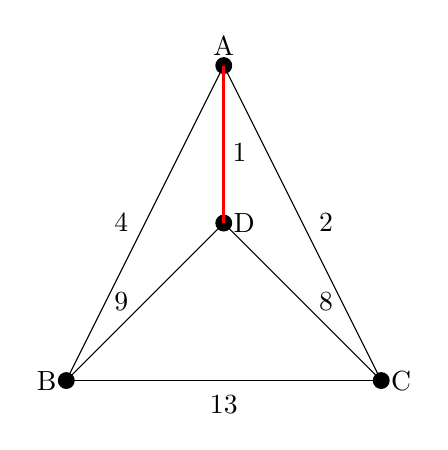
\begin{tikzpicture}
\draw[fill] (0,0) circle[radius=.1] node [left]{B};
\draw[fill] (4,0) circle[radius=.1] node [right]{C};
\draw[fill] (2,2) circle[radius=.1] node [right]{D};
\draw[fill] (2,4) circle[radius=.1] node [above]{A};
\draw(0,0)--(4,0);
\draw(0,0)--(2,2);
\draw(0,0)--(2,4);
\draw(4,0)--(2,2);
\draw(4,0)--(2,4);
\draw[very thick, red](2,4)--(2,2);
\node at (2,-0.3){13};
\node at (0.7,1){9};
\node at (0.7,2){4};
\node at (3.3,1){8};
\node at (3.3,2){2};
\node at (2.2,2.9){1};
\end{tikzpicture}
}
\end{center}
\end{minipage}
%
\begin{minipage}{.5\textwidth}
\begin{center}
\scalebox{0.8}{
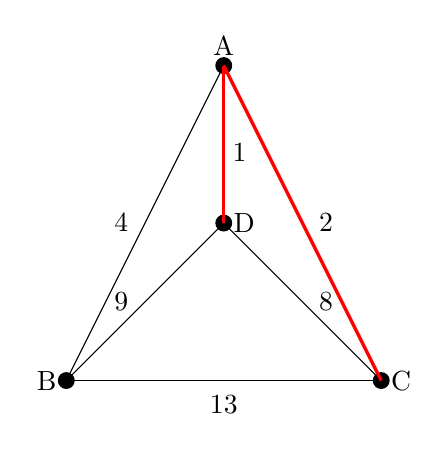
\begin{tikzpicture}
\draw[fill] (0,0) circle[radius=.1] node [left]{B};
\draw[fill] (4,0) circle[radius=.1] node [right]{C};
\draw[fill] (2,2) circle[radius=.1] node [right]{D};
\draw[fill] (2,4) circle[radius=.1] node [above]{A};
\draw(0,0)--(4,0);
\draw(0,0)--(2,2);
\draw(0,0)--(2,4);
\draw(4,0)--(2,2);
\draw[very thick, red](4,0)--(2,4);
\draw[very thick, red](2,4)--(2,2);
\node at (2,-0.3){13};
\node at (0.7,1){9};
\node at (0.7,2){4};
\node at (3.3,1){8};
\node at (3.3,2){2};
\node at (2.2,2.9){1};
\end{tikzpicture}
}
\end{center}
\end{minipage}

For the third edge, we'd like to add AB, but that would give vertex A degree 3, which is not allowed in a Hamiltonian circuit.  The next shortest edge is CD, but that edge would create a circuit ACDA that does not include vertex B, so we reject that edge.  The next shortest edge is BD, so we add that edge to the graph.

\begin{minipage}{.3\textwidth}
\begin{center}
\scalebox{.8}{
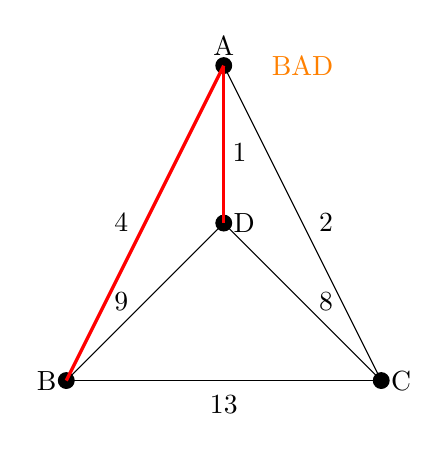
\begin{tikzpicture}
\draw[fill] (0,0) circle[radius=.1] node [left]{B};
\draw[fill] (4,0) circle[radius=.1] node [right]{C};
\draw[fill] (2,2) circle[radius=.1] node [right]{D};
\draw[fill] (2,4) circle[radius=.1] node [above]{A};
\draw(0,0)--(4,0);
\draw(0,0)--(2,2);
\draw[very thick, red](0,0)--(2,4);
\draw(4,0)--(2,2);
\draw(4,0)--(2,4);
\draw[very thick, red](2,4)--(2,2);
\node at (2,-0.3){13};
\node at (0.7,1){9};
\node at (0.7,2){4};
\node at (3.3,1){8};
\node at (3.3,2){2};
\node at (2.2,2.9){1};
\node at (3,4){\textcolor{orange}{BAD}};
\end{tikzpicture}
}
\end{center}
\end{minipage}
%
\begin{minipage}{.3\textwidth}
\begin{center}
\scalebox{0.8}{
\begin{tikzpicture}
\draw[fill] (0,0) circle[radius=.1] node [left]{B};
\draw[fill] (4,0) circle[radius=.1] node [right]{C};
\draw[fill] (2,2) circle[radius=.1] node [right]{D};
\draw[fill] (2,4) circle[radius=.1] node [above]{A};
\draw(0,0)--(4,0);
\draw(0,0)--(2,2);
\draw(0,0)--(2,4);
\draw[very thick, red](4,0)--(2,2);
\draw[very thick, red](4,0)--(2,4);
\draw[very thick, red](2,4)--(2,2);
\node at (2,-0.3){13};
\node at (0.7,1){9};
\node at (0.7,2){4};
\node at (3.3,1){8};
\node at (3.3,2){2};
\node at (2.2,2.9){1};
\node at (3,4){\textcolor{orange}{BAD}};
\end{tikzpicture}
}
\end{center}
\end{minipage}
%
\begin{minipage}{.3\textwidth}
\begin{center}
\scalebox{0.8}{
\begin{tikzpicture}
\draw[fill] (0,0) circle[radius=.1] node [left]{B};
\draw[fill] (4,0) circle[radius=.1] node [right]{C};
\draw[fill] (2,2) circle[radius=.1] node [right]{D};
\draw[fill] (2,4) circle[radius=.1] node [above]{A};
\draw(0,0)--(4,0);
\draw[very thick, red](0,0)--(2,2);
\draw(0,0)--(2,4);
\draw(4,0)--(2,2);
\draw[very thick, red](4,0)--(2,4);
\draw[very thick, red](2,4)--(2,2);
\node at (2,-0.3){13};
\node at (0.7,1){9};
\node at (0.7,2){4};
\node at (3.3,1){8};
\node at (3.3,2){2};
\node at (2.2,2.9){1};
\node at (3,4){\textcolor{teal}{GOOD}};
\end{tikzpicture}
}
\end{center}
\end{minipage}



We then add the last edge to complete the circuit: ACBDA with weight 25.  \\

\begin{center}
\scalebox{0.8}{
\begin{tikzpicture}
\draw[fill] (0,0) circle[radius=.1] node [left]{B};
\draw[fill] (4,0) circle[radius=.1] node [right]{C};
\draw[fill] (2,2) circle[radius=.1] node [right]{D};
\draw[fill] (2,4) circle[radius=.1] node [above]{A};
\draw[very thick, red](0,0)--(4,0);
\draw[very thick, red](0,0)--(2,2);
\draw(0,0)--(2,4);
\draw(4,0)--(2,2);
\draw[very thick, red](4,0)--(2,4);
\draw[very thick, red](2,4)--(2,2);
\node at (2,-0.3){13};
\node at (0.7,1){9};
\node at (0.7,2){4};
\node at (3.3,1){8};
\node at (3.3,2){2};
\node at (2.2,2.9){1};
\end{tikzpicture}
}
\end{center}

Notice that the algorithm did not produce the optimal circuit in this case; the optimal circuit is ACDBA with weight 23.  
\end{example}

While the Sorted Edge algorithm overcomes some of the shortcomings of NNA, it is still only a heuristic algorithm, and does not guarantee the optimal circuit.

\begin{example}{}{} %21
Your teacher's band, \textit{Derivative Work}, is doing a bar tour in Oregon.  The driving distances are shown below.  Plan an efficient route for your teacher to visit all the cities and return to the starting location.  Use NNA starting at Portland, and then use Sorted Edges.
\begin{center}
\begin{tabular}{|l|c|c|c|c|c|c|c|c|c|c|}
\hline
&&&&&&&&&&\\[7ex]
& \begin{rotate}{90}Ashland \end{rotate}& \begin{rotate}{90}Astoria\end{rotate}  & \begin{rotate}{90}Bend \end{rotate}& \begin{rotate}{90}Corvallis \end{rotate} & \begin{rotate}{90}Crater Lake \end{rotate} &  \begin{rotate}{90}Eugene  \end{rotate}&  \begin{rotate}{90}Newport \end{rotate} &  \begin{rotate}{90}Portland  \end{rotate}& \begin{rotate}{90}Salem \end{rotate} &  \begin{rotate}{90}Seaside \end{rotate}\\
\hline
Ashland & --&374&200&223&108&178&252&285&240&356\\
\hline
Astoria & 374&--&255&166&433&199&135&95&136&17\\
\hline
Bend & 200 & 255 &--&128&277&128&180 & 160&131&247\\
\hline
Corvalis&223&166&128&--&430&47&52&84&40&155\\
\hline
Crater Lake &108&433&277&430&--&453&478&344&389&423\\
\hline
Eugene &178&199&128&47&453&--&91&110&64&181\\
\hline
Newport&252&135&180&52&478&91&--&114&83&117\\
\hline
Portland &285&95&160&84&344&110&114&--&47&78\\
\hline
Salem & 240 &136&131&40&389&64&83&47&--&118\\
\hline
Seaside&356&17&247&155&423&181&117&78&118&--\\
\hline
\end{tabular}
\end{center}



\noindent Using NNA with a large number of cities, you might find it helpful to mark off the cities as they're visited to keep from accidentaly visiting them again.  Looking in the row for Portland, the smallest distance is 47, to Salem.  Following that idea, our circuit will be:\\
\begin{minipage}{0.5\textwidth}
\begin{tabular}{ll}
Portland to Salem&		47\\
Salem to Corvallis&		40\\
Corvallis to Eugene&		47\\
Eugene to Newport	&	91\\
Newport to Seaside	&	117\\
Seaside to Astoria	&	17\\
Astoria to Bend		&255\\
Bend to Ashland	&	200\\
Ashland to Crater Lake&	108\\
Crater Lake to Portland&	344\\
Total trip length:		&1266 miles\\
\end{tabular}\\


Using Sorted Edges, you might find it helpful to draw an empty graph, perhaps by drawing vertices in a circular pattern.  Adding edges to the graph as you select them will help you visualize any circuits or vertices with degree 3.\\
\end{minipage}
%
\begin{minipage}{0.5\textwidth}
\vspace{0.5in}
\scalebox{0.7}{
\begin{tikzpicture}
\draw[fill] (2,-2) circle[radius=.1] node[below]{Portland};
\draw[fill] (1,0) circle[radius=.1] node[above]{Salem};
\draw[fill] (9,0) circle[radius=.1] node[above]{Corvalis};
\draw[fill] (2,2) circle[radius=.1] node[above]{Seaside};
\draw[fill] (4,3) circle[radius=.1] node[above]{Ashland};
\draw[fill] (4,-3) circle[radius=.1] node[below]{Newport};
\draw[fill] (6,3) circle[radius=.1] node[above]{Astoria};
\draw[fill] (6,-3) circle[radius=.1] node[below]{Eugene};
\draw[fill] (8,2) circle[radius=.1] node[above]{Bend};
\draw[fill] (8,-2) circle[radius=.1] node[below]{Crater Lake};
\end{tikzpicture}
}
\end{minipage}

\begin{minipage}{0.5\textwidth}
We start adding the shortest edges:\\
\begin{tabular}{ll}
Seaside to Astoria&	17 miles\\
Corvallis to Salem	&40 miles\\
Portland to Salem	&47 miles\\
Corvallis to Eugene	&47 miles\\
\end{tabular}\\

The graph after adding these edges is shown to the right.   The next shortest edge is from Corvallis to Newport at 52 miles, but adding that edge would give Corvallis degree 3.  \\
\end{minipage}
%
\begin{minipage}{0.5\textwidth}
\scalebox{0.7}{
\begin{tikzpicture}
\draw[fill] (2,-2) circle[radius=.1] node[below]{Portland};
\draw[fill] (1,0) circle[radius=.1] node[above]{Salem};
\draw[fill] (9,0) circle[radius=.1] node[above]{Corvalis};
\draw[fill] (2,2) circle[radius=.1] node[above]{Seaside};
\draw[fill] (4,3) circle[radius=.1] node[above]{Ashland};
\draw[fill] (4,-3) circle[radius=.1] node[below]{Newport};
\draw[fill] (6,3) circle[radius=.1] node[above]{Astoria};
\draw[fill] (6,-3) circle[radius=.1] node[below]{Eugene};
\draw[fill] (8,2) circle[radius=.1] node[above]{Bend};
\draw[fill] (8,-2) circle[radius=.1] node[below]{Crater Lake};
\draw(2,2)--(6,3);
\draw(1,0)--(9,0);
\draw(1,0)--(2,-2);
\draw(9,0)--(6,-3);
\end{tikzpicture}
}
\end{minipage}

\begin{minipage}{0.5\textwidth}
Continuing on, we can skip over any edge pair that contains Salem or Corvallis, since they both already have degree 2.\\
\begin{tabular}{ll}
Portland to Seaside& 		78 miles\\
Eugene to Newport	&	91 miles\\
Portland to Astoria	&	(reject -- closes circuit)\\
Ashland to Crater Lake	&108 miles\\
\end{tabular}\\

\noindent The graph after adding these edges is shown to the right.  At this point, we can skip over any edge pair that contains Salem, Seaside, Eugene, Portland, or Corvallis since they already have degree 2.\\
\end{minipage}
%
\begin{minipage}{0.5\textwidth}
\scalebox{0.7}{
\begin{tikzpicture}
\draw[fill] (2,-2) circle[radius=.1] node[below]{Portland};
\draw[fill] (1,0) circle[radius=.1] node[above]{Salem};
\draw[fill] (9,0) circle[radius=.1] node[above]{Corvallis};
\draw[fill] (2,2) circle[radius=.1] node[above]{Seaside};
\draw[fill] (4,3) circle[radius=.1] node[above]{Ashland};
\draw[fill] (4,-3) circle[radius=.1] node[below]{Newport};
\draw[fill] (6,3) circle[radius=.1] node[above]{Astoria};
\draw[fill] (6,-3) circle[radius=.1] node[below]{Eugene};
\draw[fill] (8,2) circle[radius=.1] node[above]{Bend};
\draw[fill] (8,-2) circle[radius=.1] node[below]{Crater Lake};
\draw(2,2)--(6,3);
\draw(1,0)--(9,0);
\draw(1,0)--(2,-2);
\draw(9,0)--(6,-3);
\draw(2,2)--(2,-2);
\draw(4,-3)--(6,-3);
\draw(8,-2)--(4,3);
\end{tikzpicture}
}
\end{minipage}


\begin{minipage}{0.5\textwidth}
\begin{tabular}{ll}
Newport to Astoria	&	(reject -- closes circuit)\\
Newport to Bend	&	180 miles\\
Bend to Ashland	&	200 miles\\
\end{tabular}

At this point the only way to complete the circuit is to add:
\begin{tabular}{ll}
Crater Lake to Astoria	&433 miles\\
\end{tabular}

\noindent The final circuit, written to start at Portland, is:
Portland, Salem, Corvallis, Eugene, Newport, Bend, Ashland, Crater Lake, Astoria, Seaside, Portland.
\end{minipage}
%
\begin{minipage}{0.5\textwidth}
\scalebox{0.7}{
\begin{tikzpicture}
\draw[fill] (2,-2) circle[radius=.1] node[below]{Portland};
\draw[fill] (1,0) circle[radius=.1] node[above]{Salem};
\draw[fill] (9,0) circle[radius=.1] node[above]{Corvallis};
\draw[fill] (2,2) circle[radius=.1] node[above]{Seaside};
\draw[fill] (4,3) circle[radius=.1] node[above]{Ashland};
\draw[fill] (4,-3) circle[radius=.1] node[below]{Newport};
\draw[fill] (6,3) circle[radius=.1] node[above]{Astoria};
\draw[fill] (6,-3) circle[radius=.1] node[below]{Eugene};
\draw[fill] (8,2) circle[radius=.1] node[above]{Bend};
\draw[fill] (8,-2) circle[radius=.1] node[below]{Crater Lake};
\draw(2,2)--(6,3);
\draw(1,0)--(9,0);
\draw(1,0)--(2,-2);
\draw(9,0)--(6,-3);
\draw(2,2)--(2,-2);
\draw(4,-3)--(6,-3);
\draw(8,-2)--(4,3);
\draw(6,3)--(8,-2);
\draw(8,2)--(4,-3);
\draw(8,2)--(4,3);
\end{tikzpicture}
}
\end{minipage}

\noindent Total trip length:  1241 miles.\\

\noindent While better than the NNA route, neither algorithm produced the optimal route.  The following route can make the tour in 1069 miles:  Portland, Astoria, Seaside, Newport, Corvallis, Eugene, Ashland, Crater Lake, Bend, Salem, Portland.
\end{example}



\begin{exercise}{}{} %6
Find the circuit produced by the Sorted Edges algorithm using the graph below.\\
\begin{tikzpicture}
\draw[fill] (0,0) circle[radius=.1] node[left]{A};
\draw[fill] (2,2) circle[radius=.1] node[above]{B};
\draw[fill] (2,-2) circle[radius=.1] node[below]{C};
\draw[fill] (4,2) circle[radius=.1] node[above]{E};
\draw[fill] (4,-2) circle[radius=.1] node[below]{F};
\draw[fill] (6,0) circle[radius=.1] node[right]{G};
\draw(0,0) to node[above]{11} (2,2);
\draw(0,0) to node[below]{33}(2,-2);
\draw(0,0) to node[pos=0.3, fill=ocre!10]{14}(4,2);
\draw(0,0) to node[pos=0.3, fill=ocre!10]{41}(4,-2);
\draw(0,0) to node[near start, fill=ocre!10]{27}(6,0);
\draw(2,2) to node[pos=0.37, fill=ocre!10]{25}(2,-2);
\draw(2,2) to node[above]{43}(4,2);
\draw(2,2) to node[pos=0.7, fill=ocre!10]{23}(4,-2);
\draw(2,2) to node[pos=0.7, fill=ocre!10]{13}(6,0);
\draw(2,-2) to node[pos=0.35, fill=ocre!10]{17} (4,2);
\draw(2,-2) to node[below]{37}(4,-2);
\draw(2,-2) to node[pos=0.7, fill=ocre!10]{36}(6,0);
\draw(4,2) to node[pos=0.38, fill=ocre!10]{15}(4,-2);
\draw(4,2) to node[above]{45}(6,0);
\draw(4,-2) to node[below]{19}(6,0);
\end{tikzpicture}
\end{exercise}

\section{Spanning Trees}
A company requires reliable internet and phone connectivity between their five offices (named A, B, C, D, and E for simplicity) in New York, so they decide to lease dedicated lines from the phone company.  The phone company will charge for each link made.  The costs, in thousands of dollars per year, are shown in the graph.

\begin{center}
\begin{tikzpicture}
\draw[fill] (0,0) circle[radius=.1] node[below]{D};
\draw[fill] (3,0) circle[radius=.1] node[below]{C};
\draw[fill] (-1,1.5) circle[radius=.1] node[left]{E};
\draw[fill] (2,3) circle[radius=.1] node[above]{A};
\draw[fill] (5,1.5) circle[radius=.1] node[right]{B};
\draw(0,0)--(3,0);
\draw(0,0)--(2,3);
\draw(0,0)--(-1,1.5);
\draw(0,0)--(5,1.5);
\draw(3,0)--(-1,1.5);
\draw(3,0)--(2,3);
\draw(3,0)--(5,1.5);
\draw(-1,1.5)--(2,3);
\draw(-1,1.5)--(5,1.5);
\draw(2,3)--(5,1.5);
\node at (1.5, -0.2){\$7};
\node at (-0.9, 0.7){\$13};
\node at (4.6,0.7){\$10};
\node at (3.5, 2.5){\$4};
\node at (0.5,2.5){\$5};
\node at (1.7,1.3){\$6};
\node at (1.15,2.15){\$9};
\node at (2.5,2.15){\$8};
\node at (0,0.9){\$11};
\node at (3.4,0.85){\$14};
\end{tikzpicture}
\end{center}

In this case, we don't need to find a circuit, or even a specific path; all we need to do is make sure we can make a call from any office to any other.  In other words, we need to be sure there is a path from any vertex to any other vertex.


\begin{definition}{Spanning Tree}{}
A spanning tree is a connected graph using all vertices in which there are no circuits.  
In other words, there is a path from any vertex to any other vertex, but no circuits.   
\end{definition}

Some examples of spanning trees are shown below.  Notice there are no circuits in the trees, and it is fine to have vertices with degree higher than two.\\

\begin{minipage}{0.2\textwidth}
\begin{tikzpicture}
\draw[fill] (0,0) circle[radius=.1];
\draw[fill] (1,1) circle[radius=.1];
\draw[fill] (1,2) circle[radius=.1];
\draw[fill] (2,0) circle[radius=.1];
\draw(0,0)--(1,2);
\draw(0,0)--(1,1);
\draw(1,2)--(2,0);
\end{tikzpicture}
\end{minipage}
%
\begin{minipage}{0.2\textwidth}
\begin{tikzpicture}
\draw[fill] (0,0) circle[radius=.1];
\draw[fill] (1,1) circle[radius=.1];
\draw[fill] (1,2) circle[radius=.1];
\draw[fill] (2,0) circle[radius=.1];
\draw(0,0)--(1,2);
\draw(2,0)--(1,1);
\draw(1,2)--(2,0);
\end{tikzpicture}
\end{minipage}
%
\begin{minipage}{0.2\textwidth}
\begin{tikzpicture}
\draw[fill] (0,0) circle[radius=.1];
\draw[fill] (1,1) circle[radius=.1];
\draw[fill] (1,2) circle[radius=.1];
\draw[fill] (2,0) circle[radius=.1];
\draw(0,0)--(1,2);
\draw(0,0)--(1,1);
\draw(0,0)--(2,0);
\end{tikzpicture}
\end{minipage}
%
\begin{minipage}{0.2\textwidth}
\begin{tikzpicture}
\draw[fill] (0,0) circle[radius=.1];
\draw[fill] (1,1) circle[radius=.1];
\draw[fill] (1,2) circle[radius=.1];
\draw[fill] (2,0) circle[radius=.1];
\draw(0,0)--(1,2);
\draw(1,2)--(1,1);
\draw(1,2)--(2,0);
\end{tikzpicture}
\end{minipage}
%
\begin{minipage}{0.2\textwidth}
\begin{tikzpicture}
\draw[fill] (0,0) circle[radius=.1];
\draw[fill] (1,1) circle[radius=.1];
\draw[fill] (1,2) circle[radius=.1];
\draw[fill] (2,0) circle[radius=.1];
\draw(1,1)--(1,2);
\draw(1,2)--(2,0);
\draw(0,0)--(2,0);
\end{tikzpicture}
\end{minipage}\\

Usually we have a starting graph to work from, like in the phone example above.  In this case, we form our spanning tree by finding a \textbf{subgraph} -- a new graph formed using all the vertices but only some of the edges from the original graph.  No edges will be created where they didn't already exist.

Of course, any random spanning tree isn't really what we want.  We want the \textbf{minimum cost spanning tree (MCST)}.

\begin{definition}{Minimum Cost Spanning Tree (MCST)}{}
The minimum cost spanning tree is the spanning tree with the smallest total edge weight.  
\end{definition}


A nearest neighbor style approach doesn't make as much sense here since we don't need a circuit, so instead we will take an approach similar to sorted edges.

\begin{algorithm}{}{}[Kruskal's Algorithm]
\hspace{3in}
\begin{enumerate}
\item Select the cheapest unused edge in the graph.
\item Repeat step 1, adding the cheapest unused edge, unless:
\begin{itemize}
\item adding the edge would create a circuit.
\end{itemize}
\item Repeat until a spanning tree is formed.
\end{enumerate}
\end{algorithm}



\begin{example}{}{} %22
Using our phone line graph from above, begin adding edges:\\
\begin{minipage}{.5\textwidth}
\begin{tabular}{lll}
AB&	\$4&	OK\\
AE	&\$5	&OK\\
BE	&\$6&	reject -- closes circuit ABEA\\
DC	&\$7&	OK\\
AC&\$8&	OK\\
\end{tabular}
\end{minipage}
%
\begin{minipage}{.5\textwidth}
\begin{tikzpicture}
\draw[fill] (0,0) circle[radius=.1] node[below]{D};
\draw[fill] (3,0) circle[radius=.1] node[below]{C};
\draw[fill] (-1,1.5) circle[radius=.1] node[left]{E};
\draw[fill] (2,3) circle[radius=.1] node[above]{A};
\draw[fill] (5,1.5) circle[radius=.1] node[right]{B};
\draw[very thick, red](0,0)--(3,0);
\draw(0,0)--(2,3);
\draw(0,0)--(-1,1.5);
\draw(0,0)--(5,1.5);
\draw(3,0)--(-1,1.5);
\draw[very thick, red](3,0)--(2,3);
\draw(3,0)--(5,1.5);
\draw[very thick, red](-1,1.5)--(2,3);
\draw(-1,1.5)--(5,1.5);
\draw[very thick, red](2,3)--(5,1.5);
\node at (1.5, -0.2){\$7};
\node at (-0.9, 0.7){\$13};
\node at (4.6,0.7){\$10};
\node at (3.5, 2.5){\$4};
\node at (0.5,2.5){\$5};
\node at (1.7,1.3){\$6};
\node at (1.15,2.15){\$9};
\node at (2.5,2.15){\$8};
\node at (0,0.9){\$11};
\node at (3.4,0.85){\$14};
\end{tikzpicture}
\end{minipage}

At this point we stop -- every vertex is now connected, so we have formed a spanning tree with cost \$24 thousand a year.
\end{example}

Remarkably, Kruskal's algorithm is both optimal and efficient; we are guaranteed to always produce the optimal MCST.


\begin{example}{}{} %23
The power company needs to lay updated distribution lines connecting the ten Oregon cities below to the power grid.  How can they minimize the amount of new line to lay?
 
\begin{center}
\begin{tabular}{|l|c|c|c|c|c|c|c|c|c|c|}
\hline
&&&&&&&&&&\\[7ex]
& \begin{rotate}{90}Ashland \end{rotate}& \begin{rotate}{90}Astoria\end{rotate}  & \begin{rotate}{90}Bend \end{rotate}& \begin{rotate}{90}Corvallis \end{rotate} & \begin{rotate}{90}Crater Lake \end{rotate} &  \begin{rotate}{90}Eugene  \end{rotate}&  \begin{rotate}{90}Newport \end{rotate} &  \begin{rotate}{90}Portland  \end{rotate}& \begin{rotate}{90}Salem \end{rotate} &  \begin{rotate}{90}Seaside \end{rotate}\\
\hline
Ashland & --&374&200&223&108&178&252&285&240&356\\
\hline
Astoria & 374&--&255&166&433&199&135&95&136&17\\
\hline
Bend & 200 & 255 &--&128&277&128&180 & 160&131&247\\
\hline
Corvalis&223&166&128&--&430&47&52&84&40&155\\
\hline
Crater Lake &108&433&277&430&--&453&478&344&389&423\\
\hline
Eugene &178&199&128&47&453&--&91&110&64&181\\
\hline
Newport&252&135&180&52&478&91&--&114&83&117\\
\hline
Portland &285&95&160&84&344&110&114&--&47&78\\
\hline
Salem & 240 &136&131&40&389&64&83&47&--&118\\
\hline
Seaside&356&17&247&155&423&181&117&78&118&--\\
\hline
\end{tabular}
\end{center}

Using Kruskal's algorithm, we add edges from cheapest to most expensive, rejecting any that close a circuit.  We stop when the graph is connected.\\

\begin{minipage}{0.5\textwidth}
\begin{tabular}{ll}
Seaside to Astoria&		17 miles\\
Corvallis to Salem	&	40 miles\\
Portland to Salem	&	47 miles\\
Corvallis to Eugene	&	47 miles\\
Corvallis to Newport	&	52 miles\\
Salem to Eugene	&	reject -- closes circuit\\
Portland to Seaside	&	78 miles\\
\end{tabular}\\

The graph up to this point is shown to the right.
\end{minipage}
%
\begin{minipage}{0.5\textwidth}
\scalebox{0.7}{
\begin{tikzpicture}
\draw[fill] (2,-2) circle[radius=.1] node[below]{Portland};
\draw[fill] (1,0) circle[radius=.1] node[above]{Salem};
\draw[fill] (9,0) circle[radius=.1] node[above]{Corvalis};
\draw[fill] (2,2) circle[radius=.1] node[above]{Seaside};
\draw[fill] (4,3) circle[radius=.1] node[above]{Ashland};
\draw[fill] (4,-3) circle[radius=.1] node[below]{Newport};
\draw[fill] (6,3) circle[radius=.1] node[above]{Astoria};
\draw[fill] (6,-3) circle[radius=.1] node[below]{Eugene};
\draw[fill] (8,2) circle[radius=.1] node[above]{Bend};
\draw[fill] (8,-2) circle[radius=.1] node[below]{Crater Lake};
\draw(1,0)--(9,0);
\draw(1,0)--(2,-2);
\draw(2,2)--(6,3);
\draw(9,0)--(4,-3);
\draw(9,0)--(6,-3);
\end{tikzpicture}
}
\end{minipage}

Continuing,

\begin{minipage}{0.5\textwidth}
\begin{tabular}{ll}
Newport to Salem&		reject \\
Corvallis to Portland&		reject\\ 
Eugene to Newport	&	reject\\
Portland to Astoria	&	reject\\
Ashland to Crater Lake	&	108 miles\\
Eugene to Portland	&	reject \\
Newport to Portland	&	reject\\
Newport to Seaside	&	reject \\
Salem to Seaside	&	reject\\
Bend to Eugene	&	128 miles\\
Bend to Salem		&	reject \\
Astoria to Newport 	&	reject \\
Salem to Astoria 	&	reject \\
Corvallis to Seaside	&	reject \\
Portland to Bend	&	reject \\
Astoria to Corvallis	&	reject \\
Eugene to Ashland	&	178 miles\\
\end{tabular}\\

This connects the graph.  The total length of cable to lay would be 695 miles.
\end{minipage}
%
\begin{minipage}{0.5\textwidth}
\vspace{1in}
\scalebox{0.7}{
\begin{tikzpicture}
\draw[fill] (2,-2) circle[radius=.1] node[below]{Portland};
\draw[fill] (1,0) circle[radius=.1] node[above]{Salem};
\draw[fill] (9,0) circle[radius=.1] node[above]{Corvalis};
\draw[fill] (2,2) circle[radius=.1] node[above]{Seaside};
\draw[fill] (4,3) circle[radius=.1] node[above]{Ashland};
\draw[fill] (4,-3) circle[radius=.1] node[below]{Newport};
\draw[fill] (6,3) circle[radius=.1] node[above]{Astoria};
\draw[fill] (6,-3) circle[radius=.1] node[below]{Eugene};
\draw[fill] (8,2) circle[radius=.1] node[above]{Bend};
\draw[fill] (8,-2) circle[radius=.1] node[below]{Crater Lake};
\draw(1,0)--(9,0);
\draw(1,0)--(2,-2);
\draw(2,2)--(6,3);
\draw(9,0)--(4,-3);
\draw(9,0)--(6,-3);
\draw(8,-2)--(4,3);
\draw(4,3)--(6,-3);
\draw(6,-3)--(8,2);
\end{tikzpicture}
}
\end{minipage}

\end{example}



\begin{exercise}{}{} %7
Find a minimum cost spanning tree on the graph below using Kruskal's algorithm.\\
\begin{tikzpicture}
\draw[fill] (0,0) circle[radius=.1] node[left]{A};
\draw[fill] (2,2) circle[radius=.1] node[above]{B};
\draw[fill] (2,-2) circle[radius=.1] node[below]{C};
\draw[fill] (4,2) circle[radius=.1] node[above]{E};
\draw[fill] (4,-2) circle[radius=.1] node[below]{F};
\draw[fill] (6,0) circle[radius=.1] node[right]{G};
\draw(0,0) to node[above]{11} (2,2);
\draw(0,0) to node[below]{33}(2,-2);
\draw(0,0) to node[pos=0.3, fill=ocre!10]{14}(4,2);
\draw(0,0) to node[pos=0.3, fill=ocre!10]{41}(4,-2);
\draw(0,0) to node[near start, fill=ocre!10]{15}(6,0);
\draw(2,2) to node[pos=0.37, fill=ocre!10]{25}(2,-2);
\draw(2,2) to node[above]{43}(4,2);
\draw(2,2) to node[pos=0.7, fill=ocre!10]{23}(4,-2);
\draw(2,2) to node[pos=0.7, fill=ocre!10]{13}(6,0);
\draw(2,-2) to node[pos=0.35, fill=ocre!10]{17} (4,2);
\draw(2,-2) to node[below]{37}(4,-2);
\draw(2,-2) to node[pos=0.7, fill=ocre!10]{36}(6,0);
\draw(4,2) to node[pos=0.38, fill=ocre!10]{16}(4,-2);
\draw(4,2) to node[above]{45}(6,0);
\draw(4,-2) to node[below]{19}(6,0);
\end{tikzpicture}
\end{exercise}





\section{Exercise Answers}
\begin{enumerate}
\item  \begin{enumerate}
\item 5 vertices, 10 edges
\item Yes, it is connected.
\item The vertex is degree 4.
\item A path
\item  A circuit\\
\end{enumerate}

\item The shortest path is ABDEG, with length 13.\\

\item Yes, all vertices have even degree so this graph has an Euler Circuit.  There are several possibilities.  One is:  ABEGFCDFEDBCA\\


\item \hspace{.2in}\\
\begin{minipage}{0.5\textwidth}
This graph can be eulerized by duplicating the edge BC, as shown.  One possible Euler circuit on the eulerized graph is ACDBCBA.
\end{minipage}
%
\begin{minipage}{0.5\textwidth}
\scalebox{.7}{
\begin{tikzpicture}
\draw[fill] (0,0) circle[radius=.1] node [left]{B};
\draw[fill] (4,0) circle[radius=.1] node [right]{C};
\draw[fill] (2,2) circle[radius=.1] node [above]{D};
\draw[fill] (2,4) circle[radius=.1] node [above]{A};
\draw(0,0)--(4,0);
\draw(0,0)--(2,2);
\draw(0,0)--(2,4);
\draw(4,0)--(2,2);
\draw(4,0)--(2,4);
\draw[very thick, red](0,0) to [bend right] (4,0);
\end{tikzpicture}
}
\end{minipage}

\item At each step, we look for the nearest location we haven't already visited.  \\
From B the nearest computer is E with time 24.  \\
From E, the nearest computer is D with time 11.  \\
From D the nearest is A with time 12. \\
From A the nearest is C with time 34.  \\
From C, the only computer we haven't visited is F with time 27.\\
From F, we return back to B with time 50.\\

\noindent The NNA circuit from B is BEDACFB with time 158 milliseconds.\\

\noindent Using NNA again from other starting vertices:\\
Starting at A: ADEBCFA: time 146\\
Starting at C: CDEBAFC: time 167\\
Starting at D: DEBCFAD: time 146\\
Starting at E: EDACFBE: time 158\\
Starting at F: FDEBCAF: time 158\\

\noindent The RNNA found a circuit with time 146 milliseconds:  ADEBCFA.  We could also write this same circuit starting at B if we wanted:  BCFADEB or BEDAFCB.\\

\item \hspace{.2in}\\
\begin{minipage}{0.5\textwidth}
AB: Add, cost 11\\
BG: Add, cost 13\\
AE: Add, cost 14\\
EF: Add, cost 15\\
EC: Skip (degree 3 at E)\\
FG: Skip (would create a circuit not including C)\\
BF, BC, AG, AC: Skip (would cause a vertex to have degree 3)\\
GC: Add, cost 36\\
CF: Add, cost 37, completes the circuit\\

\noindent Final circuit:  ABGCFEA\\
\end{minipage}
%
\begin{minipage}{0.5\textwidth}
\begin{tikzpicture}
\draw[fill] (0,0) circle[radius=.1] node[left]{A};
\draw[fill] (2,2) circle[radius=.1] node[above]{B};
\draw[fill] (2,-2) circle[radius=.1] node[below]{C};
\draw[fill] (4,2) circle[radius=.1] node[above]{E};
\draw[fill] (4,-2) circle[radius=.1] node[below]{F};
\draw[fill] (6,0) circle[radius=.1] node[right]{G};
\draw[very thick, red](0,0) to node[above]{11} (2,2);
\draw(0,0) to node[below]{33}(2,-2);
\draw[very thick, red](0,0) to node[pos=0.3, fill=white]{14}(4,2);
\draw(0,0) to node[pos=0.3, fill=white]{41}(4,-2);
\draw(0,0) to node[near start, fill=white]{27}(6,0);
\draw(2,2) to node[pos=0.37, fill=white]{25}(2,-2);
\draw(2,2) to node[above]{43}(4,2);
\draw(2,2) to node[pos=0.7, fill=white]{23}(4,-2);
\draw[very thick, red](2,2) to node[pos=0.7, fill=white]{13}(6,0);
\draw(2,-2) to node[pos=0.35, fill=white]{17} (4,2);
\draw[very thick, red](2,-2) to node[below]{37}(4,-2);
\draw[very thick, red](2,-2) to node[pos=0.7, fill=white]{36}(6,0);
\draw[very thick, red](4,2) to node[pos=0.38, fill=white]{15}(4,-2);
\draw(4,2) to node[above]{45}(6,0);
\draw(4,-2) to node[below]{19}(6,0);
\end{tikzpicture}
\end{minipage}

\item \hspace{.2in}\\
\begin{minipage}{0.5\textwidth}
AB: Add, cost 11\\
BG: Add, cost 13\\
AE: Add, cost 14\\
AG: Skip, would create circuit ABGA\\
EF: Add, cost 16\\
EC: Add, cost 17\\

\noindent This completes the spanning tree.\\
\end{minipage}
%
\begin{minipage}{0.5\textwidth}
\begin{tikzpicture}
\draw[fill] (0,0) circle[radius=.1] node[left]{A};
\draw[fill] (2,2) circle[radius=.1] node[above]{B};
\draw[fill] (2,-2) circle[radius=.1] node[below]{C};
\draw[fill] (4,2) circle[radius=.1] node[above]{E};
\draw[fill] (4,-2) circle[radius=.1] node[below]{F};
\draw[fill] (6,0) circle[radius=.1] node[right]{G};
\draw[very thick, red](0,0) to node[above]{11} (2,2);
\draw(0,0) to node[below]{33}(2,-2);
\draw[very thick, red](0,0) to node[pos=0.3, fill=white]{14}(4,2);
\draw(0,0) to node[pos=0.3, fill=white]{41}(4,-2);
\draw(0,0) to node[near start, fill=white]{15}(6,0);
\draw(2,2) to node[pos=0.37, fill=white]{25}(2,-2);
\draw(2,2) to node[above]{43}(4,2);
\draw(2,2) to node[pos=0.7, fill=white]{23}(4,-2);
\draw[very thick, red](2,2) to node[pos=0.7, fill=white]{13}(6,0);
\draw[very thick, red](2,-2) to node[pos=0.35, fill=white]{17} (4,2);
\draw(2,-2) to node[below]{37}(4,-2);
\draw(2,-2) to node[pos=0.7, fill=white]{36}(6,0);
\draw[very thick, red](4,2) to node[pos=0.38, fill=white]{16}(4,-2);
\draw(4,2) to node[above]{45}(6,0);
\draw(4,-2) to node[below]{19}(6,0);
\end{tikzpicture}

\end{minipage}
\end{enumerate}
\section{Additional Exercises}

\textbf{Skills}
\begin{enumerate}
\item	To deliver mail in a particular neighborhood, the postal carrier needs to walk along each of the streets with houses (the dots).  Create a graph with edges showing where the carrier must walk to deliver the mail.\\

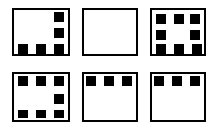
\includegraphics{graph-theory-graphics/GraphExercise1.png}\\

\item	Suppose that a town has 7 bridges as pictured below.  Create a graph that could be used to determine if there is a path that crosses all bridges once.\\

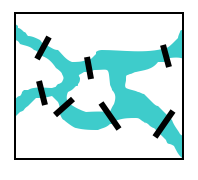
\includegraphics{graph-theory-graphics/GraphExercise2.png}\\

\item	The table below shows approximate driving times (in minutes, without traffic) between five cities in the Dallas area.  Create a weighted graph representing this data.
\begin{center}
\begin{tabular}{|l|c|c|c|c|}
\hline
&Plano&Mesquite&Arlington&Denton\\
\hline
Fort Worth&54&52&19&42\\
\hline
Plano&&38&53&41\\
\hline
Mesquite&&&43&56\\
\hline
Arlington&&&&50\\
\hline
\end{tabular}
\end{center}

\item	Shown in the table below are the one-way airfares between 5 cities\footnote{Cheapest fares found when retrieved Sept. 1, 2009 for travel Sept. 22, 2009}.  Create a graph showing this data.
\begin{center}
\begin{tabular}{|l|c|c|c|c|}
\hline
&Honolulu&London&Moscow&Cairo\\
\hline
Seattle &\$159 &\$370&\$654&\$684\\
\hline
Honolulu&&\$830&\$854&\$801\\
\hline
London&&&\$245&\$323\\
\hline
Moscow&&&&\$329\\
\hline
\end{tabular}
\end{center}

\item	Find the degree of each vertex in the graph below.\\

\begin{tikzpicture}
\draw[fill] (0,0) circle[radius=.1];
\draw[fill] (1,0) circle[radius=.1];
\draw[fill] (0,1) circle[radius=.1];
\draw[fill] (1,1) circle[radius=.1];
\draw[fill] (2,1) circle[radius=.1];
\draw(0,0)--(1,0);
\draw(1,0)--(1,1);
\draw(1,0)--(0,1);
\draw(1,1)--(0,1);
\draw(1,1)--(2,1);
\draw(2,1)--(1,0);
\end{tikzpicture}

\item	Find the degree of each vertex in the graph below.\\

\begin{tikzpicture}
\draw[fill] (0,0) circle[radius=.1];
\draw[fill] (-1,1) circle[radius=.1];
\draw[fill] (-.5,2) circle[radius=.1];
\draw[fill] (1,1) circle[radius=.1];
\draw[fill] (.5,2) circle[radius=.1];
\draw(0,0)--(-1,1);
\draw(0,0)--(1,1);
\draw(-1,1)--(1,1);
\draw(-1,1)--(-0.5,2);
\draw(1,1)--(0.5,2);
\end{tikzpicture}

\item	Which of these graphs are connected?\\

\begin{tabular}{|c|c|c|}
\hline
&&\\
\begin{tikzpicture}
\draw[fill] (0,0) circle[radius=.1];
\draw[fill] (1,0) circle[radius=.1];
\draw[fill] (0,1) circle[radius=.1];
\draw[fill] (1,1) circle[radius=.1];
\draw[fill] (2,1) circle[radius=.1];
\draw(0,0)--(1,0);
\draw(1,0)--(1,1);
\draw(0,1)--(1,1);
\draw(1,0)--(2,1);
\end{tikzpicture}
&
\begin{tikzpicture}
\draw[fill] (0,0) circle[radius=.1];
\draw[fill] (1,0) circle[radius=.1];
\draw[fill] (0,1) circle[radius=.1];
\draw[fill] (1,1) circle[radius=.1];
\draw[fill] (2,1) circle[radius=.1];
\draw(1,0)--(1,1);
\draw(1,0)--(2,1);
\draw(1,1)--(2,1);
\draw(0,0)--(0,1);
\end{tikzpicture}
&
\begin{tikzpicture}
\draw[fill] (0,0) circle[radius=.1];
\draw[fill] (1,0) circle[radius=.1];
\draw[fill] (0,1) circle[radius=.1];
\draw[fill] (1,1) circle[radius=.1];
\draw[fill] (2,1) circle[radius=.1];
\draw(0,0)--(1,0);
\draw(1,0)--(1,1);
\draw(0,1)--(1,1);
\draw(1,0)--(2,1);
\draw(1,1)--(2,1);
\draw(0,0)--(0,1);
\end{tikzpicture}\\
&&\\
\hline
\end{tabular}\\


\item Which of these graphs are connected?\\

\begin{tabular}{|c|c|c|}
\hline
&&\\
\begin{tikzpicture}
\draw[fill] (0,0) circle[radius=.1];
\draw[fill] (1,0) circle[radius=.1];
\draw[fill] (2,0) circle[radius=.1];
\draw[fill] (.5,1) circle[radius=.1];
\draw[fill] (1.5,1) circle[radius=.1];
\draw[fill] (0,2) circle[radius=.1];
\draw[fill] (1,2) circle[radius=.1];
\draw[fill] (2,2) circle[radius=.1];
\draw(0,0)--(1,0);
\draw(1,0)--(2,0);
\draw(0.5,1)--(1.5,1);
\draw(0,2)--(1,2);
\draw(1,2)--(2,2);
\end{tikzpicture}
&
\begin{tikzpicture}
\draw[fill] (0,0) circle[radius=.1];
\draw[fill] (1,0) circle[radius=.1];
\draw[fill] (2,0) circle[radius=.1];
\draw[fill] (.5,1) circle[radius=.1];
\draw[fill] (1.5,1) circle[radius=.1];
\draw[fill] (0,2) circle[radius=.1];
\draw[fill] (1,2) circle[radius=.1];
\draw[fill] (2,2) circle[radius=.1];
\draw(0,0)--(1,0);
\draw(1,0)--(1.5,1);
\draw(0.5,1)--(1.5,1);
\draw(0,2)--(0.5,1);
\draw(1,2)--(2,2);
\draw(1.5,1)--(2,2);
\draw(1.5,1)--(2,0);
\end{tikzpicture}
&
\begin{tikzpicture}
\draw[fill] (0,0) circle[radius=.1];
\draw[fill] (1,0) circle[radius=.1];
\draw[fill] (2,0) circle[radius=.1];
\draw[fill] (.5,1) circle[radius=.1];
\draw[fill] (1.5,1) circle[radius=.1];
\draw[fill] (0,2) circle[radius=.1];
\draw[fill] (1,2) circle[radius=.1];
\draw[fill] (2,2) circle[radius=.1];
\draw(0,0)--(1,0);
\draw(1,0)--(1.5,1);
\draw(0.5,1)--(1.5,1);
\draw(0,2)--(0,0);
\draw(1,2)--(2,2);
\draw(2,2)--(2,0);
\draw(0,2)--(.5,1);
\end{tikzpicture}\\
&&\\
\hline
\end{tabular}\\

\item	Travel times by rail for a segment of the Eurail system is shown below with travel times in hours and minutes.  Find path with shortest travel time from Bern to Berlin by applying Dijkstra's algorithm.\\

\begin{tikzpicture}
\draw[fill] (0,0) circle[radius=.1] node[left]{Paris};
\draw[fill] (2,-3) circle[radius=.1] node[left]{Lyon};
\draw[fill] (4,-2.5) circle[radius=.1] node[below]{Bern};
\draw[fill] (6,-1.5) circle[radius=.1] node[left]{Frankfurt};
\draw[fill] (8,-2) circle[radius=.1] node[below]{M\"unchen};
\draw[fill] (4.5,2) circle[radius=.1] node[above]{Amsterdam};
\draw[fill] (7,2) circle[radius=.1] node[above]{Berlin};
\draw(0,0) to node[above]{1:25} (4.5,2);
\draw(0,0) to node[left]{1:55} (2,-3);
\draw(2,-3) to node[below]{3:50} (4,-2.5);
\draw(4,-2.5) to node[left]{3.55} (6,-1.5);
\draw(6,-1.5) to node[above]{3:10} (8,-2);
\draw(6,-1.5) to node[left]{4:00} (4.5,2);
\draw(8,-2) to node[right]{5:45} (7,2);
\draw(7,2) to node[below]{6:10} (4.5,2);
\end{tikzpicture}


\item	Using the graph from the previous problem, find the path with shortest travel time from Paris to M\"unchen.

\item	Does each of these graphs have an Euler circuit?  If so, find it.\\

\begin{tabular}{|c|c|c|}
\hline
&&\\
\begin{tikzpicture}
\draw[fill] (0,0) circle[radius=.1];
\draw[fill] (1,1) circle[radius=.1];
\draw[fill] (2,0) circle[radius=.1];
\draw[fill] (0,2) circle[radius=.1];
\draw[fill] (2,2) circle[radius=.1];
\draw(0,0)--(2,0);
\draw(0,0)--(1,1);
\draw(1,1)--(0,2);
\draw(0,2)--(2,2);
\draw(1,1)--(2,2);
\draw(1,1)--(2,0);
\end{tikzpicture}
&
\begin{tikzpicture}
\draw[fill] (0,0) circle[radius=.1];
\draw[fill] (1,1) circle[radius=.1];
\draw[fill] (1,0) circle[radius=.1];
\draw[fill] (2,0) circle[radius=.1];
\draw[fill] (1,-1) circle[radius=.1];
\draw[fill] (2,-1) circle[radius=.1];
\draw(0,0)--(1,0);
\draw(1,0)--(2,0);
\draw(0,0)--(1,1);
\draw(1,1)--(1,0);
\draw(1,0)--(1,-1);
\draw(1,1)--(2,0);
\draw(1,-1)--(2,0);
\draw(2,0)--(2,-1);
\draw(2,-1)--(1,-1);
\draw(0,0)--(1,-1);
\end{tikzpicture}
&
\begin{tikzpicture}
\draw[fill] (0,0) circle[radius=.1];
\draw[fill] (1,1) circle[radius=.1];
\draw[fill] (2,0) circle[radius=.1];
\draw[fill] (0,2) circle[radius=.1];
\draw[fill] (2,2) circle[radius=.1];
\draw(0,0) to [bend right](1,1);
\draw(0,0) to [bend left](1,1);
\draw(1,1)--(0,2);
\draw(0,0)--(2,0);
\draw(1,1)--(2,2);
\draw(0,2)--(2,2);
\draw(2,0)--(2,2);
\draw(0,0)--(0,2);
\draw(1,1)--(2,0);
\end{tikzpicture}\\
&&\\
\hline
\end{tabular}\\


\item	Does each of these graphs have an Euler circuit?  If so, find it.\\

\begin{tabular}{|c|c|c|}
\hline
&&\\
\begin{tikzpicture}
\draw[fill] (0,0) circle[radius=.1];
\draw[fill] (2,1) circle[radius=.1];
\draw[fill] (4,0) circle[radius=.1];
\draw[fill] (1,-2) circle[radius=.1];
\draw[fill] (3,-2) circle[radius=.1];
\draw(0,0)--(2,1)--(4,0)--(3,-2)--(1,-2)--(0,0)--(4,0)--(1,-2)--(2,1)--(3,-2)--(0,0);
\end{tikzpicture}
&
\begin{tikzpicture}
\draw[fill] (0,0) circle[radius=.1];
\draw[fill] (2,0) circle[radius=.1];
\draw[fill] (4,0) circle[radius=.1];
\draw[fill] (1,1) circle[radius=.1];
\draw[fill] (3,1) circle[radius=.1];
\draw[fill] (2,2) circle[radius=.1];
\draw(0,0)--(2,0)--(4,0)--(3,1)--(2,0)--(1,1)--(0,0);
\draw(1,1)--(3,1)--(2,2)--(1,1);

\end{tikzpicture}
&
\begin{tikzpicture}
\draw[fill] (0,0) circle[radius=.1];
\draw[fill] (3,0) circle[radius=.1];
\draw[fill] (0,2) circle[radius=.1];
\draw[fill] (3,2) circle[radius=.1];
\draw[fill] (1.5,1) circle[radius=.1];
\draw(0,0)--(3,0)--(3,2)--(0,2)--(0,0);
\draw(0,2)--(1.5,1)--(3,2);

\end{tikzpicture}\\
&&\\
\hline
\end{tabular}\\


\item	Eulerize this graph using as few edge duplications as possible.  Then, find an Euler circuit.\\

\begin{tikzpicture}
\draw[fill] (0,0) circle[radius=.1];
\draw[fill] (1,0) circle[radius=.1];
\draw[fill] (2,0) circle[radius=.1];
\draw[fill] (0,1) circle[radius=.1];
\draw[fill] (1,1) circle[radius=.1];
\draw[fill] (2,1) circle[radius=.1];
\draw[fill] (0,2) circle[radius=.1];
\draw[fill] (1,2) circle[radius=.1];
\draw[fill] (2,2) circle[radius=.1];
\draw[fill] (0,3) circle[radius=.1];
\draw[fill] (1,3) circle[radius=.1];
\draw[fill] (2,3) circle[radius=.1];
\draw(0,0)--(1,0)--(2,0)--(2,1)--(1,1)--(0,1)--(0,2)--(1,2)--(2,2)--(2,3)--(1,3)--(0,3)--(0,2);
\draw(1,3)--(1,2)--(1,1)--(1,0);
\draw(0,0)--(0,1);
\draw(2,1)--(2,2);
\end{tikzpicture}

\item	Eulerize this graph using as few edge duplications as possible.  Then, find an Euler circuit.\\

\begin{tikzpicture}
\draw[fill] (0,0) circle[radius=.1];
\draw[fill] (2,0) circle[radius=.1];
\draw[fill] (4,0) circle[radius=.1];
\draw[fill] (6,0) circle[radius=.1];
\draw[fill] (0,1) circle[radius=.1];
\draw[fill] (2,1) circle[radius=.1];
\draw[fill] (4,1) circle[radius=.1];
\draw[fill] (6,1) circle[radius=.1];
\draw[fill] (0,2) circle[radius=.1];
\draw[fill] (2,2) circle[radius=.1];
\draw[fill] (4,2) circle[radius=.1];
\draw[fill] (6,2) circle[radius=.1];
\draw[fill] (0,3) circle[radius=.1];
\draw[fill] (2,3) circle[radius=.1];
\draw[fill] (4,3) circle[radius=.1];
\draw[fill] (6,3) circle[radius=.1];
\draw(0,0)--(2,0)--(4,0)--(6,0)--(6,1)--(6,2)--(6,3)--(4,3)--(2,3)--(0,3)--(0,2)--(2,2)--(2,1)--(0,1)--(0,0);
\draw(2,0)--(2,1)--(4,1)--(6,1);
\draw(2,2)--(2,3);
\draw(4,3)--(4,2)--(4,1);
\draw(4,2)--(6,2);
\end{tikzpicture}



\item	The maintenance staff at an amusement park need to patrol the major walkways, shown in the graph below, collecting litter.  Find an efficient patrol route by finding an Euler circuit.  If necessary, eulerize the graph in an efficient way.\\

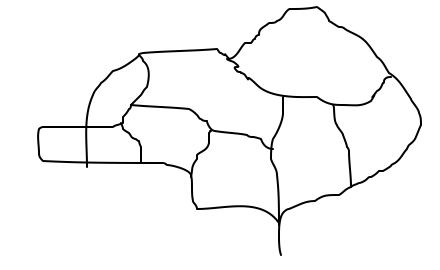
\includegraphics{graph-theory-graphics/GraphExercise15.png}\\

\item	After a storm, the city crew inspects for trees or brush blocking the road.  Find an efficient route for the neighborhood below by finding an Euler circuit.  If necessary, eulerize the graph in an efficient way.\\

\begin{tikzpicture}
\draw[fill] (1,0) circle[radius=.1];
\draw[fill] (2,0) circle[radius=.1];
\draw[fill] (3,0) circle[radius=.1];
\draw[fill] (4,0) circle[radius=.1];
\draw[fill] (5,0) circle[radius=.1];
\draw[fill] (6,0) circle[radius=.1];
\draw[fill] (0,1) circle[radius=.1];
\draw[fill] (1,1) circle[radius=.1];
\draw[fill] (4,1) circle[radius=.1];
\draw[fill] (5,1) circle[radius=.1];
\draw[fill] (0,2) circle[radius=.1];
\draw[fill] (1,2) circle[radius=.1];
\draw[fill] (2,2) circle[radius=.1];
\draw[fill] (3,2) circle[radius=.1];
\draw[fill] (0,3) circle[radius=.1];
\draw[fill] (1,3) circle[radius=.1];
\draw[fill] (2,3) circle[radius=.1];
\draw[fill] (3,3) circle[radius=.1];
\draw(1,0)--(2,0)--(3,0)--(4,0)--(5,0)--(6,0)--(5,1)--(4,1)--(5,0);
\draw(4,1)--(3,2)--(2,2)--(2,0);
\draw(1,0)--(1,1)--(0,1)--(0,2)--(0,3)--(1,3)--(2,3)--(3,3)--(3,2);
\draw (1,3)--(1,2)--(1,1);
\draw(1,2)--(2,2);
\end{tikzpicture}

\item	Does each of these graphs have at least one Hamiltonian circuit?  If so, find one. \\

\begin{tabular}{|c|c|c|}
\hline
&&\\
\begin{tikzpicture}
\draw[fill] (0,0) circle[radius=.1];
\draw[fill] (1,1) circle[radius=.1];
\draw[fill] (2,0) circle[radius=.1];
\draw[fill] (0,2) circle[radius=.1];
\draw[fill] (2,2) circle[radius=.1];
\draw(0,0)--(2,0);
\draw(0,0)--(1,1);
\draw(1,1)--(0,2);
\draw(0,2)--(2,2);
\draw(1,1)--(2,2);
\draw(1,1)--(2,0);
\end{tikzpicture}
&
\begin{tikzpicture}
\draw[fill] (0,0) circle[radius=.1];
\draw[fill] (1.5,0) circle[radius=.1];
\draw[fill] (3,0) circle[radius=.1];
\draw[fill] (0,2) circle[radius=.1];
\draw[fill] (1.5,2) circle[radius=.1];
\draw[fill] (3,2) circle[radius=.1];
\draw(0,0)--(0,2);
\draw(0,0)--(1.5,2);
\draw(0,0)--(3,2);
\draw(1.5,0)--(0,2);
\draw(1.5,0)--(1.5,2);
\draw(1.5,0)--(3,2);
\draw(3,0)--(0,2);
\draw(3,0)--(1.5,2);
\draw(3,0)--(3,2);
\end{tikzpicture}
&
\begin{tikzpicture}
\draw[fill] (0,0) circle[radius=.1];
\draw[fill] (1,0) circle[radius=.1];
\draw[fill] (2,0) circle[radius=.1];
\draw[fill] (0,1) circle[radius=.1];
\draw[fill] (1,1) circle[radius=.1];
\draw[fill] (2,1) circle[radius=.1];
\draw[fill] (1,2) circle[radius=.1];
\draw(0,0)--(1,0)--(2,0)--(2,1)--(1,2)--(0,1)--(0,0);
\draw(0,1)--(1,0)--(2,1)--(1,1)--(0,1);
\end{tikzpicture}\\
&&\\
\hline
\end{tabular}\\

\item	Does each of these graphs have at least one Hamiltonian circuit?  If so, find one. \\

\begin{tabular}{|c|c|c|}
\hline
&&\\
\begin{tikzpicture}
\draw[fill] (0,0) circle[radius=.1];
\draw[fill] (2,0) circle[radius=.1];
\draw[fill] (0,2) circle[radius=.1];
\draw[fill] (2,2) circle[radius=.1];
\draw[fill] (.7,.7) circle[radius=.1];
\draw[fill] (1.4,.7) circle[radius=.1];
\draw[fill] (.7,1.4) circle[radius=.1];
\draw[fill] (1.4,1.4) circle[radius=.1];
\draw(0,0)--(2,0)--(2,2)--(0,2)--(0,0);
\draw(.7,.7)--(1.4,.7)--(1.4,1.4)--(.7,1.4)--(.7,.7);
\draw(0,0)--(.7,.7);
\draw(2,0)--(1.4,.7);
\draw(2,2)--(1.4,1.4);
\draw(0,2)--(.7,1.4);
\end{tikzpicture}
&
\begin{tikzpicture}
\draw[fill] (0,0) circle[radius=.1];
\draw[fill] (1.5,0) circle[radius=.1];
\draw[fill] (3,0) circle[radius=.1];
\draw[fill] (0.75,2) circle[radius=.1];
\draw[fill] (2.25,2) circle[radius=.1];
\draw(0,0)--(0.75,2);
\draw(0,0)--(2.25,2);
\draw(1.5,0)--(0.75,2);
\draw(1.5,0)--(2.25,2);
\draw(3,0)--(0.75,2);
\draw(3,0)--(2.25,2);
\end{tikzpicture}
&
\begin{tikzpicture}
\draw[fill] (0,0) circle[radius=.1];
\draw[fill] (1,1) circle[radius=.1];
\draw[fill] (1,0) circle[radius=.1];
\draw[fill] (2,0) circle[radius=.1];
\draw[fill] (1,-1) circle[radius=.1];
\draw[fill] (2,-1) circle[radius=.1];
\draw(0,0)--(1,0);
\draw(1,0)--(2,0);
\draw(0,0)--(1,1);
\draw(1,1)--(1,0);
\draw(1,0)--(1,-1);
\draw(1,1)--(2,0);
\draw(1,-1)--(2,0);
\draw(2,0)--(2,-1);
\draw(2,-1)--(1,-1);
\draw(0,0)--(1,-1);
\end{tikzpicture}
\\
\hline
\end{tabular}\\

\item	A company needs to deliver product to each of their 5 stores around the Dallas, TX area.  Driving distances between the stores are shown below.  Find a route for the driver to follow, returning to the distribution center in Fort Worth:
\begin{enumerate}
\item	Using Nearest Neighbor starting in Fort Worth
\item	Using Repeated Nearest Neighbor
\item	Using Sorted Edges
\end{enumerate}
\begin{center}
\begin{tabular}{|l|c|c|c|c|}
\hline
&Plano&Mesquite&Arlington&Denton\\
\hline
Fort Worth&54&52&19&42\\
\hline
Plano&&38&53&41\\
\hline
Mesquite&&&43&56\\
\hline
Arlington&&&&50\\
\hline
\end{tabular}
\end{center}

\item	A salesperson needs to travel from Seattle to Honolulu, London, Moscow, and Cairo.  Use the table of flight costs from problem \#4 to find a route for this person to follow:
\begin{enumerate}
\item	Using Nearest Neighbor starting in Seattle
\item	Using Repeated Nearest Neighbor
\item	Using Sorted Edges\\
\end{enumerate}

\item	When installing fiber optics, some companies will install a sonet ring; a full loop of cable connecting multiple locations.  This is used so that if any part of the cable is damaged it does not interrupt service, since there is a second connection to the hub.  A company has 5 buildings.  Costs (in thousands of dollars) to lay cables between pairs of buildings are shown below.   Find the circuit that will minimize cost:
\begin{enumerate}
\item	Using Nearest Neighbor starting at building A
\item	Using Repeated Nearest Neighbor
\item	Using Sorted Edges\\
\end{enumerate}

\begin{tikzpicture}
\draw(0,0)  to node[fill=white]{\$5.6}(3,0);
\draw(0,0)  to node[near end, fill=white]{\$5.1}(2,3);
\draw(0,0)  to node[fill=white]{\$6.0}(-1,1.5);
\draw(3,0)  to node[pos=0.49,fill=white]{\$4.3}(-1,1.5);
\draw(3,0)  to node[pos=0.6, fill=white]{\$4.7}(2,3);
\draw(3,0) to node[pos=0.3, fill=white]{\$5.8}(5,1.5);
\draw(-1,1.5) to node[fill=white]{\$5.9}(2,3);
\draw(-1,1.5)  to node[pos=0.2, fill=white]{\$5.2}(5,1.5);
\draw(2,3)  to node[fill=white]{\$4.4}(5,1.5);
\draw(0,0) to node[pos=0.7, fill=white]{\$4.0}(5,1.5);
\draw[fill] (0,0) circle[radius=.1] node[below]{C};
\draw[fill] (3,0) circle[radius=.1] node[below]{D};
\draw[fill] (-1,1.5) circle[radius=.1] node[left]{B};
\draw[fill] (2,3) circle[radius=.1] node[above]{A};
\draw[fill] (5,1.5) circle[radius=.1] node[right]{E};
\end{tikzpicture}\\



\item	A tourist wants to visit 7 cities in Israel.  Driving distances, in kilometers, between the cities are shown below\footnote{From \url{http://www.ddtravel-acc.com/Israel-cities-distance.htm}}.  Find a route for the person to follow, returning to the starting city:
\begin{enumerate}
\item	Using Nearest Neighbor starting in Jerusalem
\item	Using Repeated Nearest Neighbor
\item	Using Sorted Edges
\end{enumerate}
\begin{center}
\begin{tabular}{|l|c|c|c|c|c|c|}
\hline
&Jerusalem&Tel Aviv&Haifa&Tiberias&Beer Sheba&Eilat\\
\hline
Jerusalem&--&&&&&\\
\hline
Tel Aviv&58&--&&&&\\
\hline
Haifa&151&95&--&&&\\
\hline
Tiberias&152&134&69&--&&\\
\hline
Beer Sheba&81&105&197&233&--&\\
\hline
Eilat&309&346&438&405&241&--\\
\hline
Nazareth&131&102&35&29&207&488\\
\hline
\end{tabular}
\end{center}


\item	Find a minimum cost spanning tree for the graph you created in problem \#3.\\

\item	Find a minimum cost spanning tree for the graph you created in problem \#22.\\

\item	Find a minimum cost spanning tree for the graph from problem \#21.\\
\end{enumerate}

\noindent \textbf{Concepts}

\begin{enumerate}[start=26]
\item Can a graph have one vertex with odd degree?  If not, are there other values that are not possible?  Why?\\

\item	A complete graph is one in which there is an edge connecting every vertex to every other vertex.  For what values of n does complete graph with n vertices have an Euler circuit?  A Hamiltonian circuit?

\item Create a graph by drawing $n$ vertices in a row, then another $n$ vertices below those.  Draw an edge from each vertex in the top row to every vertex in the bottom row.  An example when $n=3$ is shown below.  For what values of $n$ will a graph created this way have an Euler circuit?  A Hamiltonian circuit?\\

\begin{tikzpicture}
\draw[fill] (0,0) circle[radius=.1];
\draw[fill] (2,0) circle[radius=.1];
\draw[fill] (4,0) circle[radius=.1];
\draw[fill] (0,2) circle[radius=.1];
\draw[fill] (2,2) circle[radius=.1];
\draw[fill] (4,2) circle[radius=.1];
\draw(0,0)--(0,2);
\draw(0,0)--(2,2);
\draw(0,0)--(4,2);
\draw(2,0)--(0,2);
\draw(2,0)--(2,2);
\draw(2,0)--(4,2);
\draw(4,0)--(0,2);
\draw(4,0)--(2,2);
\draw(4,0)--(4,2);
\end{tikzpicture}\\

\item	Eulerize this graph in the most efficient way possible, considering the weights of the edges.\\

\begin{tikzpicture}
\draw[fill] (0,0) circle[radius=.1];
\draw[fill] (2,0) circle[radius=.1];
\draw[fill] (5,0) circle[radius=.1];
\draw[fill] (7,0) circle[radius=.1];
\draw[fill] (0,1) circle[radius=.1];
\draw[fill] (2,1) circle[radius=.1];
\draw[fill] (5,1) circle[radius=.1];
\draw[fill] (7,1) circle[radius=.1];
\draw[fill] (0,2) circle[radius=.1];
\draw[fill] (2,2) circle[radius=.1];
\draw[fill] (5,2) circle[radius=.1];
\draw[fill] (7,2) circle[radius=.1];
\draw(0,0) to node[above]{2}(2,0);
\draw(2,0)to node[above]{3}(5,0);
\draw(5,0) to node[above]{2}(7,0);
\draw(0,1) to node[above]{2}(2,1);
\draw(2,1)to node[above]{3}(5,1);
\draw(5,1) to node[above]{2}(7,1);
\draw(0,2) to node[above]{2}(2,2);
\draw(2,2)to node[above]{3}(5,2);
\draw(5,2)to node[above]{2}(7,2);
\draw(0,0) to node[left]{1}(0,1);
\draw(0,1) to node[left]{1}(0,2);
\draw(2,0) to node[left]{1}(2,1);
\draw(2,1) to node[left]{1}(2,2);
\draw(5,0) to node[left]{1}(5,1);
\draw(5,1) to node[left]{1}(5,2);
\draw(7,0) to node[left]{1}(7,1);
\draw(7,1) to node[left]{1}(7,2);
\end{tikzpicture}\\

\item Eulerize this graph in the most efficient way possible, considering the weights of the edges.\\

\begin{tikzpicture}
\draw[fill] (0,0) circle[radius=.1];
\draw[fill] (2,0) circle[radius=.1];
\draw[fill] (6,0) circle[radius=.1];
\draw[fill] (8,0) circle[radius=.1];
\draw[fill] (0,1) circle[radius=.1];
\draw[fill] (2,1) circle[radius=.1];
\draw[fill] (6,1) circle[radius=.1];
\draw[fill] (8,1) circle[radius=.1];
\draw[fill] (0,2) circle[radius=.1];
\draw[fill] (2,2) circle[radius=.1];
\draw[fill] (6,2) circle[radius=.1];
\draw[fill] (8,2) circle[radius=.1];
\draw[fill] (0,3) circle[radius=.1];
\draw[fill] (2,3) circle[radius=.1];
\draw[fill] (6,3) circle[radius=.1];
\draw[fill] (8,3) circle[radius=.1];
\draw(0,0) to node[above]{2}(2,0);
\draw(2,0)to node[above]{4}(6,0);
\draw(6,0) to node[above]{2}(8,0);
\draw(0,1) to node[above]{2}(2,1);
\draw(2,1)to node[above]{4}(6,1);
\draw(6,1) to node[above]{2}(8,1);
\draw(0,2) to node[above]{2}(2,2);
\draw(2,2)to node[above]{4}(6,2);
\draw(6,2)to node[above]{2}(8,2);
\draw(0,3) to node[above]{2}(2,3);
\draw(2,3)to node[above]{4}(6,3);
\draw(6,3)to node[above]{2}(8,3);
\draw(0,0) to node[left]{1}(0,1);
\draw(0,1) to node[left]{1}(0,2);
\draw(2,0) to node[left]{1}(2,1);
\draw(2,1) to node[left]{1}(2,2);
\draw(6,0) to node[left]{1}(6,1);
\draw(6,1) to node[left]{1}(6,2);
\draw(8,0) to node[left]{1}(8,1);
\draw(8,1) to node[left]{1}(8,2);
\draw(0,2) to node[left]{1}(0,3);
\draw(2,2) to node[left]{1}(2,3);
\draw(6,2) to node[left]{1}(6,3);
\draw(8,2) to node[left]{1}(8,3);
\end{tikzpicture}\\


\item	Eulerize this graph in the most efficient way possible, considering the weights of the edges.\\

\begin{tikzpicture}
\draw(0,0)  to node[fill=white]{26}(3,0);
\draw(0,0)  to node[near end, fill=white]{24}(2,3);
\draw(0,0)  to node[fill=white]{44}(-1,1.5);
\draw(3,0)  to node[pos=0.49,fill=white]{46}(-1,1.5);
\draw(3,0)  to node[pos=0.42, fill=white]{60}(2,3);
\draw(3,0) to node[near start, fill=white]{28}(5,1.5);
\draw(-1,1.5) to node[fill=white]{22}(2,3);
\draw(-1,1.5)  to node[pos=0.2, fill=white]{26}(5,1.5);
\draw(2,3)  to node[fill=white]{30}(5,1.5);
\draw[fill] (0,0) circle[radius=.1] node[below]{C};
\draw[fill] (3,0) circle[radius=.1] node[below]{D};
\draw[fill] (-1,1.5) circle[radius=.1] node[left]{B};
\draw[fill] (2,3) circle[radius=.1] node[above]{A};
\draw[fill] (5,1.5) circle[radius=.1] node[right]{E};
\end{tikzpicture}\\

\item Eulerize this graph in the most efficient way possible, considering the weights of the edges.\\
\begin{tikzpicture}
\draw(0,0)  to node[fill=white]{12}(3,0);
\draw(0,0)  to node[near end, fill=white]{9}(2,3);
\draw(0,0)  to node[fill=white]{13}(-1,1.5);
\draw(0,0)  to node[near end, fill=white]{4}(5,1.5);
\draw(3,0)  to node[pos=0.49,fill=white]{11}(-1,1.5);
\draw(3,0)  to node[pos=0.42, fill=white]{8}(2,3);
\draw(2,3) to node[near start, fill=white]{10}(5,1.5);
\draw(-1,1.5) to node[fill=white]{5}(2,3);
\draw(-1,1.5)  to node[pos=0.2, fill=white]{6}(5,1.5);
\draw[fill] (0,0) circle[radius=.1] node[below]{E};
\draw[fill] (3,0) circle[radius=.1] node[below]{C};
\draw[fill] (-1,1.5) circle[radius=.1] node[left]{D};
\draw[fill] (2,3) circle[radius=.1] node[above]{A};
\draw[fill] (5,1.5) circle[radius=.1] node[right]{B};
\end{tikzpicture}\\



\end{enumerate}


\noindent \textbf{Explorations}

\begin{enumerate}[start=33]
\item Social networks such as Facebook and LinkedIn can be represented using graphs in which vertices represent people and edges are drawn between two vertices when those people are ``friends."   The table below shows a friendship table, where an X shows that two people are friends.
\begin{center}
\begin{tabular}{|c|c|c|c|c|c|c|c|c|c|}
\hline
&A&B&C&D&E&F&G&H&I\\
\hline
A & \cellcolor{yellow}&X&X&&&X&X&&\\
\hline
B& \cellcolor{yellow}& \cellcolor{yellow}&X&&X&&&&\\
\hline
C& \cellcolor{yellow}& \cellcolor{yellow}& \cellcolor{yellow}&&X&&&&\\
\hline
D& \cellcolor{yellow}& \cellcolor{yellow}& \cellcolor{yellow}& \cellcolor{yellow}&X&&&&X\\
\hline
E& \cellcolor{yellow}& \cellcolor{yellow}& \cellcolor{yellow}& \cellcolor{yellow}& \cellcolor{yellow}&&X&&X\\
\hline
F& \cellcolor{yellow}& \cellcolor{yellow}& \cellcolor{yellow}& \cellcolor{yellow}& \cellcolor{yellow}& \cellcolor{yellow}&&X&X\\
\hline
G& \cellcolor{yellow}& \cellcolor{yellow}& \cellcolor{yellow}& \cellcolor{yellow}& \cellcolor{yellow}& \cellcolor{yellow}& \cellcolor{yellow}&X&\\
\hline
H& \cellcolor{yellow}& \cellcolor{yellow}& \cellcolor{yellow}& \cellcolor{yellow}& \cellcolor{yellow}& \cellcolor{yellow}& \cellcolor{yellow}& \cellcolor{yellow}&X\\
\hline
\end{tabular}
\end{center}
\begin{enumerate}
\item	Create a graph of this friendship table
\item	Find the shortest path from A to D.  The length of this path is often called the ``degrees of separation" of the two people.
\item	Extension:  Split into groups.  Each group will pick 10 or more movies, and look up their major actors (www.imdb.com is a good source).  Create a graph with each actor as a vertex, and edges connecting two actors in the same movie (note the movie name on the edge).  Find interesting paths between actors, and quiz the other groups to see if they can guess the connections.\\
\end{enumerate}

\item	A spell checker in a word processing program makes suggestions when it finds a word not in the dictionary.  To determine what words to suggest, it tries to find similar words.  One measure of word similarity is the Levenshtein distance, which measures the number of substitutions, additions, or deletions that are required to change one word into another.   For example, the words spit and spot are a distance of 1 apart; changing spit to spot requires one substitution (i for o).   Likewise, spit is distance 1 from pit since the change requires one deletion (the s).  The word spite is also distance 1 from spit since it requires one addition (the e).  The word soot is distance 2 from spit since two substitutions would be required.
\begin{enumerate}
\item	Create a graph using words as vertices, and edges connecting words with a Levenshtein distance of 1.  Use the misspelled word ``moke" as the center, and try to find at least 10 connected dictionary words.  How might a spell checker use this graph?   
\item	Improve the method from above by assigning a weight to each edge based on the likelihood of making the substitution, addition, or deletion.  You can base the weights on any reasonable approach:  proximity of keys on a keyboard, common language errors, etc.  Use Dijkstra?s algorithm to find the length of the shortest path from each word to ``moke".  How might a spell checker use these values?   \\
\end{enumerate}


\item	The graph below contains two vertices of odd degree.  To eulerize this graph, it is necessary to duplicate edges connecting those two vertices.  
\begin{enumerate}
\item	Use Dijkstra's algorithm to find the shortest path between the two vertices with odd degree.  Does this produce the most efficient eulerization and solve the Chinese Postman Problem for this graph?\\

\begin{tikzpicture}
\draw[fill] (0,0) circle[radius=.1];
\draw[fill] (2,0) circle[radius=.1];
\draw[fill] (6,0) circle[radius=.1];
\draw[fill] (8,0) circle[radius=.1];
\draw[fill] (0,1) circle[radius=.1];
\draw[fill] (2,1) circle[radius=.1];
\draw[fill] (6,1) circle[radius=.1];
\draw[fill] (8,1) circle[radius=.1];
\draw[fill] (0,2) circle[radius=.1];
\draw[fill] (2,2) circle[radius=.1];
\draw[fill] (6,2) circle[radius=.1];
\draw[fill] (8,2) circle[radius=.1];

\draw(0,0) to node[above]{5}(2,0);
\draw(2,0)to node[above]{6}(6,0);
\draw(6,0) to node[above]{7}(8,0);
\draw(0,1) to node[above]{7}(2,1);
\draw(2,1)to node[near end, fill=white]{5}(6,1);
\draw(6,1) to node[above]{2}(8,1);
\draw(0,2) to node[above]{4}(2,2);
\draw(2,2)to node[above]{7}(6,2);
\draw(6,2)to node[above]{5}(8,2);

\draw(0,0) to node[left]{3}(0,1);
\draw(0,1) to node[left]{2}(0,2);
\draw(2,0) to node[left]{1}(2,1);
\draw(2,1) to node[left]{1}(2,2);
\draw(6,0) to node[left]{2}(6,1);
\draw(6,1) to node[left]{3}(6,2);
\draw(8,0) to node[left]{1}(8,1);
\draw(8,1) to node[left]{3}(8,2);

\draw(2,0) to node[fill=white, near start]{3} (6,2);
\draw(2,2) to node[fill=white, near start]{2} (6,0);

\end{tikzpicture}
\item	Suppose a graph has $n$ odd vertices.  Using the approach from part a, how many shortest paths would need to be considered?  Is this approach going to be efficient?
\end{enumerate}


\end{enumerate}


